% Generated by Sphinx.
\def\sphinxdocclass{report}
\documentclass[letterpaper,10pt,openany,oneside]{sphinxmanual}
\usepackage[utf8]{inputenc}
\DeclareUnicodeCharacter{00A0}{\nobreakspace}
\usepackage[T1]{fontenc}
\usepackage[english]{babel}
\usepackage{times}
\usepackage[Bjarne]{fncychap}
\usepackage{longtable}
\usepackage{sphinx}
\usepackage{multirow}
\usepackage{booktabs}
\usepackage{array}
\definecolor{nrelblue}{RGB}{0, 121, 193}
\hypersetup{linkcolor=nrelblue}
\usepackage[section]{placeins}


\title{nacellSE-and-hubSE Documentation}
\date{August 30, 2013}
\release{0.1.0}
\author{Katherine Dykes}
\newcommand{\sphinxlogo}{}
\renewcommand{\releasename}{Release}
\makeindex

\makeatletter
\def\PYG@reset{\let\PYG@it=\relax \let\PYG@bf=\relax%
    \let\PYG@ul=\relax \let\PYG@tc=\relax%
    \let\PYG@bc=\relax \let\PYG@ff=\relax}
\def\PYG@tok#1{\csname PYG@tok@#1\endcsname}
\def\PYG@toks#1+{\ifx\relax#1\empty\else%
    \PYG@tok{#1}\expandafter\PYG@toks\fi}
\def\PYG@do#1{\PYG@bc{\PYG@tc{\PYG@ul{%
    \PYG@it{\PYG@bf{\PYG@ff{#1}}}}}}}
\def\PYG#1#2{\PYG@reset\PYG@toks#1+\relax+\PYG@do{#2}}

\expandafter\def\csname PYG@tok@gd\endcsname{\def\PYG@tc##1{\textcolor[rgb]{0.63,0.00,0.00}{##1}}}
\expandafter\def\csname PYG@tok@gu\endcsname{\let\PYG@bf=\textbf\def\PYG@tc##1{\textcolor[rgb]{0.50,0.00,0.50}{##1}}}
\expandafter\def\csname PYG@tok@gt\endcsname{\def\PYG@tc##1{\textcolor[rgb]{0.00,0.25,0.82}{##1}}}
\expandafter\def\csname PYG@tok@gs\endcsname{\let\PYG@bf=\textbf}
\expandafter\def\csname PYG@tok@gr\endcsname{\def\PYG@tc##1{\textcolor[rgb]{1.00,0.00,0.00}{##1}}}
\expandafter\def\csname PYG@tok@cm\endcsname{\let\PYG@it=\textit\def\PYG@tc##1{\textcolor[rgb]{0.25,0.50,0.56}{##1}}}
\expandafter\def\csname PYG@tok@vg\endcsname{\def\PYG@tc##1{\textcolor[rgb]{0.73,0.38,0.84}{##1}}}
\expandafter\def\csname PYG@tok@m\endcsname{\def\PYG@tc##1{\textcolor[rgb]{0.13,0.50,0.31}{##1}}}
\expandafter\def\csname PYG@tok@mh\endcsname{\def\PYG@tc##1{\textcolor[rgb]{0.13,0.50,0.31}{##1}}}
\expandafter\def\csname PYG@tok@cs\endcsname{\def\PYG@tc##1{\textcolor[rgb]{0.25,0.50,0.56}{##1}}\def\PYG@bc##1{\setlength{\fboxsep}{0pt}\colorbox[rgb]{1.00,0.94,0.94}{\strut ##1}}}
\expandafter\def\csname PYG@tok@ge\endcsname{\let\PYG@it=\textit}
\expandafter\def\csname PYG@tok@vc\endcsname{\def\PYG@tc##1{\textcolor[rgb]{0.73,0.38,0.84}{##1}}}
\expandafter\def\csname PYG@tok@il\endcsname{\def\PYG@tc##1{\textcolor[rgb]{0.13,0.50,0.31}{##1}}}
\expandafter\def\csname PYG@tok@go\endcsname{\def\PYG@tc##1{\textcolor[rgb]{0.19,0.19,0.19}{##1}}}
\expandafter\def\csname PYG@tok@cp\endcsname{\def\PYG@tc##1{\textcolor[rgb]{0.00,0.44,0.13}{##1}}}
\expandafter\def\csname PYG@tok@gi\endcsname{\def\PYG@tc##1{\textcolor[rgb]{0.00,0.63,0.00}{##1}}}
\expandafter\def\csname PYG@tok@gh\endcsname{\let\PYG@bf=\textbf\def\PYG@tc##1{\textcolor[rgb]{0.00,0.00,0.50}{##1}}}
\expandafter\def\csname PYG@tok@ni\endcsname{\let\PYG@bf=\textbf\def\PYG@tc##1{\textcolor[rgb]{0.84,0.33,0.22}{##1}}}
\expandafter\def\csname PYG@tok@nl\endcsname{\let\PYG@bf=\textbf\def\PYG@tc##1{\textcolor[rgb]{0.00,0.13,0.44}{##1}}}
\expandafter\def\csname PYG@tok@nn\endcsname{\let\PYG@bf=\textbf\def\PYG@tc##1{\textcolor[rgb]{0.05,0.52,0.71}{##1}}}
\expandafter\def\csname PYG@tok@no\endcsname{\def\PYG@tc##1{\textcolor[rgb]{0.38,0.68,0.84}{##1}}}
\expandafter\def\csname PYG@tok@na\endcsname{\def\PYG@tc##1{\textcolor[rgb]{0.25,0.44,0.63}{##1}}}
\expandafter\def\csname PYG@tok@nb\endcsname{\def\PYG@tc##1{\textcolor[rgb]{0.00,0.44,0.13}{##1}}}
\expandafter\def\csname PYG@tok@nc\endcsname{\let\PYG@bf=\textbf\def\PYG@tc##1{\textcolor[rgb]{0.05,0.52,0.71}{##1}}}
\expandafter\def\csname PYG@tok@nd\endcsname{\let\PYG@bf=\textbf\def\PYG@tc##1{\textcolor[rgb]{0.33,0.33,0.33}{##1}}}
\expandafter\def\csname PYG@tok@ne\endcsname{\def\PYG@tc##1{\textcolor[rgb]{0.00,0.44,0.13}{##1}}}
\expandafter\def\csname PYG@tok@nf\endcsname{\def\PYG@tc##1{\textcolor[rgb]{0.02,0.16,0.49}{##1}}}
\expandafter\def\csname PYG@tok@si\endcsname{\let\PYG@it=\textit\def\PYG@tc##1{\textcolor[rgb]{0.44,0.63,0.82}{##1}}}
\expandafter\def\csname PYG@tok@s2\endcsname{\def\PYG@tc##1{\textcolor[rgb]{0.25,0.44,0.63}{##1}}}
\expandafter\def\csname PYG@tok@vi\endcsname{\def\PYG@tc##1{\textcolor[rgb]{0.73,0.38,0.84}{##1}}}
\expandafter\def\csname PYG@tok@nt\endcsname{\let\PYG@bf=\textbf\def\PYG@tc##1{\textcolor[rgb]{0.02,0.16,0.45}{##1}}}
\expandafter\def\csname PYG@tok@nv\endcsname{\def\PYG@tc##1{\textcolor[rgb]{0.73,0.38,0.84}{##1}}}
\expandafter\def\csname PYG@tok@s1\endcsname{\def\PYG@tc##1{\textcolor[rgb]{0.25,0.44,0.63}{##1}}}
\expandafter\def\csname PYG@tok@gp\endcsname{\let\PYG@bf=\textbf\def\PYG@tc##1{\textcolor[rgb]{0.78,0.36,0.04}{##1}}}
\expandafter\def\csname PYG@tok@sh\endcsname{\def\PYG@tc##1{\textcolor[rgb]{0.25,0.44,0.63}{##1}}}
\expandafter\def\csname PYG@tok@ow\endcsname{\let\PYG@bf=\textbf\def\PYG@tc##1{\textcolor[rgb]{0.00,0.44,0.13}{##1}}}
\expandafter\def\csname PYG@tok@sx\endcsname{\def\PYG@tc##1{\textcolor[rgb]{0.78,0.36,0.04}{##1}}}
\expandafter\def\csname PYG@tok@bp\endcsname{\def\PYG@tc##1{\textcolor[rgb]{0.00,0.44,0.13}{##1}}}
\expandafter\def\csname PYG@tok@c1\endcsname{\let\PYG@it=\textit\def\PYG@tc##1{\textcolor[rgb]{0.25,0.50,0.56}{##1}}}
\expandafter\def\csname PYG@tok@kc\endcsname{\let\PYG@bf=\textbf\def\PYG@tc##1{\textcolor[rgb]{0.00,0.44,0.13}{##1}}}
\expandafter\def\csname PYG@tok@c\endcsname{\let\PYG@it=\textit\def\PYG@tc##1{\textcolor[rgb]{0.25,0.50,0.56}{##1}}}
\expandafter\def\csname PYG@tok@mf\endcsname{\def\PYG@tc##1{\textcolor[rgb]{0.13,0.50,0.31}{##1}}}
\expandafter\def\csname PYG@tok@err\endcsname{\def\PYG@bc##1{\setlength{\fboxsep}{0pt}\fcolorbox[rgb]{1.00,0.00,0.00}{1,1,1}{\strut ##1}}}
\expandafter\def\csname PYG@tok@kd\endcsname{\let\PYG@bf=\textbf\def\PYG@tc##1{\textcolor[rgb]{0.00,0.44,0.13}{##1}}}
\expandafter\def\csname PYG@tok@ss\endcsname{\def\PYG@tc##1{\textcolor[rgb]{0.32,0.47,0.09}{##1}}}
\expandafter\def\csname PYG@tok@sr\endcsname{\def\PYG@tc##1{\textcolor[rgb]{0.14,0.33,0.53}{##1}}}
\expandafter\def\csname PYG@tok@mo\endcsname{\def\PYG@tc##1{\textcolor[rgb]{0.13,0.50,0.31}{##1}}}
\expandafter\def\csname PYG@tok@mi\endcsname{\def\PYG@tc##1{\textcolor[rgb]{0.13,0.50,0.31}{##1}}}
\expandafter\def\csname PYG@tok@kn\endcsname{\let\PYG@bf=\textbf\def\PYG@tc##1{\textcolor[rgb]{0.00,0.44,0.13}{##1}}}
\expandafter\def\csname PYG@tok@o\endcsname{\def\PYG@tc##1{\textcolor[rgb]{0.40,0.40,0.40}{##1}}}
\expandafter\def\csname PYG@tok@kr\endcsname{\let\PYG@bf=\textbf\def\PYG@tc##1{\textcolor[rgb]{0.00,0.44,0.13}{##1}}}
\expandafter\def\csname PYG@tok@s\endcsname{\def\PYG@tc##1{\textcolor[rgb]{0.25,0.44,0.63}{##1}}}
\expandafter\def\csname PYG@tok@kp\endcsname{\def\PYG@tc##1{\textcolor[rgb]{0.00,0.44,0.13}{##1}}}
\expandafter\def\csname PYG@tok@w\endcsname{\def\PYG@tc##1{\textcolor[rgb]{0.73,0.73,0.73}{##1}}}
\expandafter\def\csname PYG@tok@kt\endcsname{\def\PYG@tc##1{\textcolor[rgb]{0.56,0.13,0.00}{##1}}}
\expandafter\def\csname PYG@tok@sc\endcsname{\def\PYG@tc##1{\textcolor[rgb]{0.25,0.44,0.63}{##1}}}
\expandafter\def\csname PYG@tok@sb\endcsname{\def\PYG@tc##1{\textcolor[rgb]{0.25,0.44,0.63}{##1}}}
\expandafter\def\csname PYG@tok@k\endcsname{\let\PYG@bf=\textbf\def\PYG@tc##1{\textcolor[rgb]{0.00,0.44,0.13}{##1}}}
\expandafter\def\csname PYG@tok@se\endcsname{\let\PYG@bf=\textbf\def\PYG@tc##1{\textcolor[rgb]{0.25,0.44,0.63}{##1}}}
\expandafter\def\csname PYG@tok@sd\endcsname{\let\PYG@it=\textit\def\PYG@tc##1{\textcolor[rgb]{0.25,0.44,0.63}{##1}}}

\def\PYGZbs{\char`\\}
\def\PYGZus{\char`\_}
\def\PYGZob{\char`\{}
\def\PYGZcb{\char`\}}
\def\PYGZca{\char`\^}
\def\PYGZam{\char`\&}
\def\PYGZlt{\char`\<}
\def\PYGZgt{\char`\>}
\def\PYGZsh{\char`\#}
\def\PYGZpc{\char`\%}
\def\PYGZdl{\char`\$}
\def\PYGZti{\char`\~}
% for compatibility with earlier versions
\def\PYGZat{@}
\def\PYGZlb{[}
\def\PYGZrb{]}
\makeatother

\begin{document}

\maketitle
\tableofcontents
\phantomsection\label{index::doc}



\chapter{Introduction}
\label{intro:introduction}\label{intro:nacellese-and-hubse}\label{intro::doc}
The set of models contained in this software allow for the determination of dimensions and mass properties for major hub and drivetrain components of a wind turbine.  The software combines sources of information from several areas: The NREL Cost and Scaling Model {\hyperref[theory:1]{{[}1{]}}} and related subsequent cost model development efforts, the Wind Partnerships for Advanced Component Technology (WindPACT) work that occurred between roughly 2002 to 2005 {\hyperref[theory:2]{{[}2{]}}}, and the University of Sunderland (the Sunderland Model) {\hyperref[theory:3]{{[}3{]}}}.  The goal of the development of the following set of models for the hub and nacelle are to return to a semi-empirical physical representation of the turbine that allows one to assess the impact of design changes on mass via a few updates to the Sunderland model in key areas of limitation related to outdated design criteria.  The resulting models contain two key areas:
\begin{enumerate}
\item {} 
A physical model for sizing each of the major hub and drivetrain components based on design loads as they are transferred through the wind turbine system.

\item {} 
A model of the Mass Moments of Inertia for each of the components based on an assumption of homogenous distribution of homogeneous material throughout a simplified geometric structure.

\end{enumerate}


\chapter{Installation}
\label{installation:installation}\label{installation::doc}
\begin{notice}{note}{prerequisites}

NumPy, SciPy
\end{notice}

Download either sunderpact.py-0.1.0.tar.gz or sunderpact.py-0.1.0.zip, and uncompress/unpack it.

Install HubNacelleCST with the following command.

\begin{quote}
\begin{Verbatim}[commandchars=\\\{\}]
\PYG{n+nv}{\PYGZdl{} }python setup.py install
\end{Verbatim}
\end{quote}

To check if installation was successful run the unit tests for the NREL 5MW model

\begin{quote}
\begin{Verbatim}[commandchars=\\\{\}]
\PYG{n+nv}{\PYGZdl{} }python \PYG{n+nb}{test}/test\PYGZus{}sunderpact.py
\end{Verbatim}
\end{quote}

An `OK' signifies that all the tests passed.

To access an HTML version of this documentation which contains further details and links to the source code, open docs/index.html.


\chapter{Tutorial}
\label{tutorial:tutorial-label}\label{tutorial::doc}\label{tutorial:tutorial}
As an example, let us simulate model calculations for major wind turbine components for the NREL 5MW Reference Model {[}Jonkman2009{]}.

The first step is to import the relevant files.

\begin{quote}
\begin{Verbatim}[commandchars=\\\{\}]
\PYG{k+kn}{from} \PYG{n+nn}{sunderpact.src.hubSE} \PYG{k+kn}{import} \PYG{n}{HubSystem}
\PYG{k+kn}{from} \PYG{n+nn}{sunderpact.src.nacelleSE} \PYG{k+kn}{import} \PYG{n}{NacelleSystem}
\end{Verbatim}
\end{quote}

We will start with the hub system model.  The hub model relies on inputs from the rotor such as blade mass, rotor diameter, and blade number.  It also requires either the specification of variables necessary to calculate the maximum bending moment at the blade root (the wind speed necessary to achieve rated power production, air density conditions, and rotor solidity) or the root moment itself.  Specification of the hub diameter is an optional input.  If it is not supplied, then it will be calculated internal to the model.

\begin{quote}
\begin{Verbatim}[commandchars=\\\{\}]
\PYG{c}{\PYGZsh{} simple test of hubsystem sunderpact model}

\PYG{c}{\PYGZsh{} NREL 5 MW turbine}
\PYG{n}{BladeMass} \PYG{o}{=} \PYG{l+m+mf}{17740.0} \PYG{c}{\PYGZsh{} kg}
\PYG{n}{RotorDiam} \PYG{o}{=} \PYG{l+m+mf}{126.0} \PYG{c}{\PYGZsh{} m}
\PYG{n}{BladeNum}  \PYG{o}{=} \PYG{l+m+mi}{3}
\PYG{n}{hubDiam}   \PYG{o}{=} \PYG{l+m+mf}{0.0} \PYG{c}{\PYGZsh{} m}
\PYG{n}{RootMoment}\PYG{o}{=} \PYG{l+m+mf}{0.0} \PYG{c}{\PYGZsh{} Nm}
\PYG{n}{AirDensity}\PYG{o}{=} \PYG{l+m+mf}{1.225} \PYG{c}{\PYGZsh{} kg/(m\PYGZca{}3)}
\PYG{n}{Solidity}  \PYG{o}{=} \PYG{l+m+mf}{0.0517} 
\PYG{n}{RatedWindSpeed} \PYG{o}{=} \PYG{l+m+mf}{11.05} \PYG{c}{\PYGZsh{} m/s}
\end{Verbatim}
\end{quote}

We now instantiate the hub system object which contains a hub, pitch system and spinner component.  The initialization automatically updates the mass of the components and overall system based on the supplied inputs.  In addition, calculations of mass properties are also made.

\begin{quote}
\begin{Verbatim}[commandchars=\\\{\}]
\PYG{c}{\PYGZsh{} 4 ----------}

\PYG{k}{print} \PYG{l+s}{"}\PYG{l+s}{NREL 5 MW turbine test}\PYG{l+s}{"}
\PYG{k}{print} \PYG{l+s}{"}\PYG{l+s}{Hub Components}\PYG{l+s}{"}
\PYG{k}{print} \PYG{l+s}{'}\PYG{l+s}{  hub         \PYGZob{}0:8.1f\PYGZcb{} kg}\PYG{l+s}{'}\PYG{o}{.}\PYG{n}{format}\PYG{p}{(}\PYG{n}{hub}\PYG{o}{.}\PYG{n}{hub}\PYG{o}{.}\PYG{n}{mass}\PYG{p}{)}  \PYG{c}{\PYGZsh{} 31644.47}
\PYG{k}{print} \PYG{l+s}{'}\PYG{l+s}{  pitch mech  \PYGZob{}0:8.1f\PYGZcb{} kg}\PYG{l+s}{'}\PYG{o}{.}\PYG{n}{format}\PYG{p}{(}\PYG{n}{hub}\PYG{o}{.}\PYG{n}{pitchSystem}\PYG{o}{.}\PYG{n}{mass}\PYG{p}{)} \PYG{c}{\PYGZsh{} 17003.98}
\PYG{k}{print} \PYG{l+s}{'}\PYG{l+s}{  nose cone   \PYGZob{}0:8.1f\PYGZcb{} kg}\PYG{l+s}{'}\PYG{o}{.}\PYG{n}{format}\PYG{p}{(}\PYG{n}{hub}\PYG{o}{.}\PYG{n}{spinner}\PYG{o}{.}\PYG{n}{mass}\PYG{p}{)} \PYG{c}{\PYGZsh{} 1810.50}
\PYG{k}{print} \PYG{l+s}{'}\PYG{l+s}{HUB TOTAL     \PYGZob{}0:8.1f\PYGZcb{} kg}\PYG{l+s}{'}\PYG{o}{.}\PYG{n}{format}\PYG{p}{(}\PYG{n}{hub}\PYG{o}{.}\PYG{n}{mass}\PYG{p}{)} \PYG{c}{\PYGZsh{} 50458.95}
\PYG{k}{print} \PYG{l+s}{'}\PYG{l+s}{cm \PYGZob{}0:6.2f\PYGZcb{} \PYGZob{}1:6.2f\PYGZcb{} \PYGZob{}2:6.2f\PYGZcb{}}\PYG{l+s}{'}\PYG{o}{.}\PYG{n}{format}\PYG{p}{(}\PYG{n}{hub}\PYG{o}{.}\PYG{n}{cm}\PYG{p}{[}\PYG{l+m+mi}{0}\PYG{p}{]}\PYG{p}{,} \PYG{n}{hub}\PYG{o}{.}\PYG{n}{cm}\PYG{p}{[}\PYG{l+m+mi}{1}\PYG{p}{]}\PYG{p}{,} \PYG{n}{hub}\PYG{o}{.}\PYG{n}{cm}\PYG{p}{[}\PYG{l+m+mi}{2}\PYG{p}{]}\PYG{p}{)}
\PYG{k}{print} \PYG{l+s}{'}\PYG{l+s}{I \PYGZob{}0:6.1f\PYGZcb{} \PYGZob{}1:6.1f\PYGZcb{} \PYGZob{}2:6.1f\PYGZcb{}}\PYG{l+s}{'}\PYG{o}{.}\PYG{n}{format}\PYG{p}{(}\PYG{n}{hub}\PYG{o}{.}\PYG{n}{I}\PYG{p}{[}\PYG{l+m+mi}{0}\PYG{p}{]}\PYG{p}{,} \PYG{n}{hub}\PYG{o}{.}\PYG{n}{I}\PYG{p}{[}\PYG{l+m+mi}{1}\PYG{p}{]}\PYG{p}{,} \PYG{n}{hub}\PYG{o}{.}\PYG{n}{I}\PYG{p}{[}\PYG{l+m+mi}{2}\PYG{p}{]}\PYG{p}{)}

\PYG{c}{\PYGZsh{} 4 ---------}
\PYG{c}{\PYGZsh{} 5 ---------}

\PYG{c}{\PYGZsh{} simple test of nacelle sunderpact model}

\PYG{c}{\PYGZsh{} NREL 5 MW Rotor Variables}
\PYG{n}{RotorDiam} \PYG{o}{=} \PYG{l+m+mf}{126.0} \PYG{c}{\PYGZsh{} m}
\PYG{n}{RotorSpeed} \PYG{o}{=} \PYG{l+m+mf}{12.13} \PYG{c}{\PYGZsh{} m/s}
\PYG{n}{RotorTorque} \PYG{o}{=} \PYG{l+m+mf}{4365248.74} \PYG{c}{\PYGZsh{} Nm}
\PYG{n}{RotorThrust} \PYG{o}{=} \PYG{l+m+mf}{500930.84} \PYG{c}{\PYGZsh{} N}
\PYG{n}{RotorMass} \PYG{o}{=} \PYG{l+m+mf}{142585.75} \PYG{c}{\PYGZsh{} kg}

\PYG{c}{\PYGZsh{} NREL 5 MW Drivetrain variables}
\PYG{n}{iDsgn} \PYG{o}{=} \PYG{l+m+mi}{1} \PYG{c}{\PYGZsh{} geared 3-stage Gearbox with induction generator machine}
\PYG{n}{MachineRating} \PYG{o}{=} \PYG{l+m+mf}{5000.0} \PYG{c}{\PYGZsh{} kW}
\PYG{n}{GearRatio} \PYG{o}{=} \PYG{l+m+mf}{97.0} \PYG{c}{\PYGZsh{} 97:1 as listed in the 5 MW reference document}
\PYG{n}{GearConfig} \PYG{o}{=} \PYG{l+s}{'}\PYG{l+s}{eep}\PYG{l+s}{'} \PYG{c}{\PYGZsh{} epicyclic-epicyclic-parallel}
\PYG{n}{Bevel} \PYG{o}{=} \PYG{l+m+mi}{0} \PYG{c}{\PYGZsh{} no bevel stage}
\PYG{n}{crane} \PYG{o}{=} \PYG{n+nb+bp}{True} \PYG{c}{\PYGZsh{} onboard crane present}

\PYG{c}{\PYGZsh{} NREL 5 MW Tower Variables}
\PYG{n}{TowerTopDiam} \PYG{o}{=} \PYG{l+m+mf}{3.78} \PYG{c}{\PYGZsh{} m}

\PYG{c}{\PYGZsh{} 5 ---------}
\PYG{c}{\PYGZsh{} 6 ---------}

\PYG{n}{nace} \PYG{o}{=} \PYG{n}{NacelleSystem}\PYG{p}{(}\PYG{n}{RotorSpeed}\PYG{p}{,} \PYG{n}{RotorTorque}\PYG{p}{,} \PYG{n}{RotorThrust}\PYG{p}{,} \PYG{n}{RotorMass}\PYG{p}{,} \PYG{n}{RotorDiam}\PYG{p}{,} \PYG{n}{iDsgn}\PYG{p}{,} \PYGZbs{}
               \PYG{n}{MachineRating}\PYG{p}{,} \PYG{n}{GearRatio}\PYG{p}{,} \PYG{n}{GearConfig}\PYG{p}{,} \PYG{n}{Bevel}\PYG{p}{,} \PYG{n}{TowerTopDiam}\PYG{p}{,} \PYG{n}{crane}\PYG{p}{)}
               
\PYG{c}{\PYGZsh{} 6 ---------}
\PYG{c}{\PYGZsh{} 7 ---------}

\PYG{k}{print} \PYG{l+s}{'}\PYG{l+s}{----- NREL 5 MW Turbine -----}\PYG{l+s}{'}
\PYG{k}{print} \PYG{l+s}{'}\PYG{l+s}{Nacelle system model results}\PYG{l+s}{'}
\PYG{k}{print} \PYG{l+s}{'}\PYG{l+s}{Low speed shaft }\PYG{l+s+si}{\PYGZpc{}8.1f}\PYG{l+s}{ kg}\PYG{l+s}{'} \PYG{o}{\PYGZpc{}} \PYG{p}{(}\PYG{n}{nace}\PYG{o}{.}\PYG{n}{lss}\PYG{o}{.}\PYG{n}{mass}\PYG{p}{)}
\PYG{k}{print} \PYG{l+s}{'}\PYG{l+s}{Main bearings   }\PYG{l+s+si}{\PYGZpc{}8.1f}\PYG{l+s}{ kg}\PYG{l+s}{'} \PYG{o}{\PYGZpc{}} \PYG{p}{(}\PYG{n}{nace}\PYG{o}{.}\PYG{n}{mbg}\PYG{o}{.}\PYG{n}{mass}\PYG{p}{)}
\PYG{k}{print} \PYG{l+s}{'}\PYG{l+s}{Gearbox         }\PYG{l+s+si}{\PYGZpc{}8.1f}\PYG{l+s}{ kg}\PYG{l+s}{'} \PYG{o}{\PYGZpc{}} \PYG{p}{(}\PYG{n}{nace}\PYG{o}{.}\PYG{n}{gear}\PYG{o}{.}\PYG{n}{mass}\PYG{p}{)}
\PYG{k}{print} \PYG{l+s}{'}\PYG{l+s}{High speed shaft \PYGZam{} brakes  }\PYG{l+s+si}{\PYGZpc{}8.1f}\PYG{l+s}{ kg}\PYG{l+s}{'} \PYG{o}{\PYGZpc{}} \PYG{p}{(}\PYG{n}{nace}\PYG{o}{.}\PYG{n}{hss}\PYG{o}{.}\PYG{n}{mass}\PYG{p}{)}
\PYG{k}{print} \PYG{l+s}{'}\PYG{l+s}{Generator       }\PYG{l+s+si}{\PYGZpc{}8.1f}\PYG{l+s}{ kg}\PYG{l+s}{'} \PYG{o}{\PYGZpc{}} \PYG{p}{(}\PYG{n}{nace}\PYG{o}{.}\PYG{n}{gen}\PYG{o}{.}\PYG{n}{mass}\PYG{p}{)}
\PYG{k}{print} \PYG{l+s}{'}\PYG{l+s}{Variable speed electronics }\PYG{l+s+si}{\PYGZpc{}8.1f}\PYG{l+s}{ kg}\PYG{l+s}{'} \PYG{o}{\PYGZpc{}} \PYG{p}{(}\PYG{n}{nace}\PYG{o}{.}\PYG{n}{vspdEtronicsMass}\PYG{p}{)}
\PYG{k}{print} \PYG{l+s}{'}\PYG{l+s}{Overall mainframe }\PYG{l+s+si}{\PYGZpc{}8.1f}\PYG{l+s}{ kg}\PYG{l+s}{'} \PYG{o}{\PYGZpc{}} \PYG{p}{(}\PYG{n}{nace}\PYG{o}{.}\PYG{n}{mainframeMass}\PYG{p}{)}
\PYG{k}{print} \PYG{l+s}{'}\PYG{l+s}{     Bedplate     }\PYG{l+s+si}{\PYGZpc{}8.1f}\PYG{l+s}{ kg}\PYG{l+s}{'} \PYG{o}{\PYGZpc{}} \PYG{p}{(}\PYG{n}{nace}\PYG{o}{.}\PYG{n}{bpl}\PYG{o}{.}\PYG{n}{mass}\PYG{p}{)}
\PYG{k}{print} \PYG{l+s}{'}\PYG{l+s}{electrical connections  }\PYG{l+s+si}{\PYGZpc{}8.1f}\PYG{l+s}{ kg}\PYG{l+s}{'} \PYG{o}{\PYGZpc{}} \PYG{p}{(}\PYG{n}{nace}\PYG{o}{.}\PYG{n}{econnectionsMass}\PYG{p}{)}
\PYG{k}{print} \PYG{l+s}{'}\PYG{l+s}{HVAC system     }\PYG{l+s+si}{\PYGZpc{}8.1f}\PYG{l+s}{ kg}\PYG{l+s}{'} \PYG{o}{\PYGZpc{}} \PYG{p}{(}\PYG{n}{nace}\PYG{o}{.}\PYG{n}{hydrCoolingMass} \PYG{p}{)}
\PYG{k}{print} \PYG{l+s}{'}\PYG{l+s}{Nacelle cover:   }\PYG{l+s+si}{\PYGZpc{}8.1f}\PYG{l+s}{ kg}\PYG{l+s}{'} \PYG{o}{\PYGZpc{}} \PYG{p}{(}\PYG{n}{nace}\PYG{o}{.}\PYG{n}{nacelleCovMass}\PYG{p}{)}
\PYG{k}{print} \PYG{l+s}{'}\PYG{l+s}{Yaw system      }\PYG{l+s+si}{\PYGZpc{}8.1f}\PYG{l+s}{ kg}\PYG{l+s}{'} \PYG{o}{\PYGZpc{}} \PYG{p}{(}\PYG{n}{nace}\PYG{o}{.}\PYG{n}{yaw}\PYG{o}{.}\PYG{n}{mass}\PYG{p}{)}
\PYG{k}{print} \PYG{l+s}{'}\PYG{l+s}{Overall nacelle:  }\PYG{l+s+si}{\PYGZpc{}8.1f}\PYG{l+s}{ kg cm }\PYG{l+s+si}{\PYGZpc{}6.2f}\PYG{l+s}{ }\PYG{l+s+si}{\PYGZpc{}6.2f}\PYG{l+s}{ }\PYG{l+s+si}{\PYGZpc{}6.2f}\PYG{l+s}{ I }\PYG{l+s+si}{\PYGZpc{}6.2f}\PYG{l+s}{ }\PYG{l+s+si}{\PYGZpc{}6.2f}\PYG{l+s}{ }\PYG{l+s+si}{\PYGZpc{}6.2f}\PYG{l+s}{'} \PYG{o}{\PYGZpc{}} \PYG{p}{(}\PYG{n}{nace}\PYG{o}{.}\PYG{n}{mass}\PYG{p}{,} \PYG{n}{nace}\PYG{o}{.}\PYG{n}{cm}\PYG{p}{[}\PYG{l+m+mi}{0}\PYG{p}{]}\PYG{p}{,} \PYG{n}{nace}\PYG{o}{.}\PYG{n}{cm}\PYG{p}{[}\PYG{l+m+mi}{1}\PYG{p}{]}\PYG{p}{,} \PYG{n}{nace}\PYG{o}{.}\PYG{n}{cm}\PYG{p}{[}\PYG{l+m+mi}{2}\PYG{p}{]}\PYG{p}{,} \PYG{n}{nace}\PYG{o}{.}\PYG{n}{I}\PYG{p}{[}\PYG{l+m+mi}{0}\PYG{p}{]}\PYG{p}{,} \PYG{n}{nace}\PYG{o}{.}\PYG{n}{I}\PYG{p}{[}\PYG{l+m+mi}{1}\PYG{p}{]}\PYG{p}{,} \PYG{n}{nace}\PYG{o}{.}\PYG{n}{I}\PYG{p}{[}\PYG{l+m+mi}{2}\PYG{p}{]}  \PYG{p}{)}

\PYG{c}{\PYGZsh{} 7 ---------}
\end{Verbatim}
\end{quote}

The resulting system and component properties can then be printed.

\begin{quote}
\begin{Verbatim}[commandchars=\\\{\}]
\PYG{k}{print} \PYG{l+s}{"}\PYG{l+s}{NREL 5 MW turbine test}\PYG{l+s}{"}
\PYG{k}{print} \PYG{l+s}{"}\PYG{l+s}{Hub Components}\PYG{l+s}{"}
\PYG{k}{print} \PYG{l+s}{'}\PYG{l+s}{  hub         \PYGZob{}0:8.1f\PYGZcb{} kg}\PYG{l+s}{'}\PYG{o}{.}\PYG{n}{format}\PYG{p}{(}\PYG{n}{hub}\PYG{o}{.}\PYG{n}{hub}\PYG{o}{.}\PYG{n}{mass}\PYG{p}{)}  \PYG{c}{\PYGZsh{} 31644.47}
\PYG{k}{print} \PYG{l+s}{'}\PYG{l+s}{  pitch mech  \PYGZob{}0:8.1f\PYGZcb{} kg}\PYG{l+s}{'}\PYG{o}{.}\PYG{n}{format}\PYG{p}{(}\PYG{n}{hub}\PYG{o}{.}\PYG{n}{pitchSystem}\PYG{o}{.}\PYG{n}{mass}\PYG{p}{)} \PYG{c}{\PYGZsh{} 17003.98}
\PYG{k}{print} \PYG{l+s}{'}\PYG{l+s}{  nose cone   \PYGZob{}0:8.1f\PYGZcb{} kg}\PYG{l+s}{'}\PYG{o}{.}\PYG{n}{format}\PYG{p}{(}\PYG{n}{hub}\PYG{o}{.}\PYG{n}{spinner}\PYG{o}{.}\PYG{n}{mass}\PYG{p}{)} \PYG{c}{\PYGZsh{} 1810.50}
\PYG{k}{print} \PYG{l+s}{'}\PYG{l+s}{HUB TOTAL     \PYGZob{}0:8.1f\PYGZcb{} kg}\PYG{l+s}{'}\PYG{o}{.}\PYG{n}{format}\PYG{p}{(}\PYG{n}{hub}\PYG{o}{.}\PYG{n}{mass}\PYG{p}{)} \PYG{c}{\PYGZsh{} 50458.95}
\PYG{k}{print} \PYG{l+s}{'}\PYG{l+s}{cm \PYGZob{}0:6.2f\PYGZcb{} \PYGZob{}1:6.2f\PYGZcb{} \PYGZob{}2:6.2f\PYGZcb{}}\PYG{l+s}{'}\PYG{o}{.}\PYG{n}{format}\PYG{p}{(}\PYG{n}{hub}\PYG{o}{.}\PYG{n}{cm}\PYG{p}{[}\PYG{l+m+mi}{0}\PYG{p}{]}\PYG{p}{,} \PYG{n}{hub}\PYG{o}{.}\PYG{n}{cm}\PYG{p}{[}\PYG{l+m+mi}{1}\PYG{p}{]}\PYG{p}{,} \PYG{n}{hub}\PYG{o}{.}\PYG{n}{cm}\PYG{p}{[}\PYG{l+m+mi}{2}\PYG{p}{]}\PYG{p}{)}
\PYG{k}{print} \PYG{l+s}{'}\PYG{l+s}{I \PYGZob{}0:6.1f\PYGZcb{} \PYGZob{}1:6.1f\PYGZcb{} \PYGZob{}2:6.1f\PYGZcb{}}\PYG{l+s}{'}\PYG{o}{.}\PYG{n}{format}\PYG{p}{(}\PYG{n}{hub}\PYG{o}{.}\PYG{n}{I}\PYG{p}{[}\PYG{l+m+mi}{0}\PYG{p}{]}\PYG{p}{,} \PYG{n}{hub}\PYG{o}{.}\PYG{n}{I}\PYG{p}{[}\PYG{l+m+mi}{1}\PYG{p}{]}\PYG{p}{,} \PYG{n}{hub}\PYG{o}{.}\PYG{n}{I}\PYG{p}{[}\PYG{l+m+mi}{2}\PYG{p}{]}\PYG{p}{)}
\end{Verbatim}
\end{quote}

The results should appear as below:

\textgreater{}\textgreater{}\textgreater{}NREL 5 MW Turbine test
\textgreater{}\textgreater{}\textgreater{}Hub Components
\textgreater{}\textgreater{}\textgreater{}hub         29536.2 kg
\textgreater{}\textgreater{}\textgreater{}pitch mech  16670.5 kg
\textgreater{}\textgreater{}\textgreater{}nose cone    1810.5 kg
\textgreater{}\textgreater{}\textgreater{}Hub system total 48017.1 kg
\textgreater{}\textgreater{}\textgreater{}    cm -6.30 0.00 3.15
\textgreater{}\textgreater{}\textgreater{}    I 55039.9 55039.9 55039.9

Secondly, we will demonstrate the nacelle system model.  The hub model relies on inputs from the rotor and hub as well as design variables for the drivetrain. Inputs from the rotor include the rotor diameter, the rotor speed at rated power, the rotor torque at rated power, the maximum thrust from the rotor and the overall rotor mass (including blades and hub).  For the drivetrain, the overall configuration (3-stage geared, single-stage, multi-generator, or direct-drive) must be specified.  The overall gear ratio (1 for direct drive) must be specified along with the gear configuration (may be null for direct drive) and a Boolean for the presence of a bevel stage.  If an onboard crane is present, then the crane Boolean should be set true.  Finally the machine rating (in kW) must be provided.

\begin{quote}
\begin{Verbatim}[commandchars=\\\{\}]
\PYG{c}{\PYGZsh{} simple test of nacelle sunderpact model}

\PYG{c}{\PYGZsh{} NREL 5 MW Rotor Variables}
\PYG{n}{RotorDiam} \PYG{o}{=} \PYG{l+m+mf}{126.0} \PYG{c}{\PYGZsh{} m}
\PYG{n}{RotorSpeed} \PYG{o}{=} \PYG{l+m+mf}{12.13} \PYG{c}{\PYGZsh{} m/s}
\PYG{n}{RotorTorque} \PYG{o}{=} \PYG{l+m+mf}{4365248.74} \PYG{c}{\PYGZsh{} Nm}
\PYG{n}{RotorThrust} \PYG{o}{=} \PYG{l+m+mf}{500930.84} \PYG{c}{\PYGZsh{} N}
\PYG{n}{RotorMass} \PYG{o}{=} \PYG{l+m+mf}{142585.75} \PYG{c}{\PYGZsh{} kg}

\PYG{c}{\PYGZsh{} NREL 5 MW Drivetrain variables}
\PYG{n}{iDsgn} \PYG{o}{=} \PYG{l+m+mi}{1} \PYG{c}{\PYGZsh{} geared 3-stage Gearbox with induction generator machine}
\PYG{n}{MachineRating} \PYG{o}{=} \PYG{l+m+mf}{5000.0} \PYG{c}{\PYGZsh{} kW}
\PYG{n}{GearRatio} \PYG{o}{=} \PYG{l+m+mf}{97.0} \PYG{c}{\PYGZsh{} 97:1 as listed in the 5 MW reference document}
\PYG{n}{GearConfig} \PYG{o}{=} \PYG{l+s}{'}\PYG{l+s}{eep}\PYG{l+s}{'} \PYG{c}{\PYGZsh{} epicyclic-epicyclic-parallel}
\PYG{n}{Bevel} \PYG{o}{=} \PYG{l+m+mi}{0} \PYG{c}{\PYGZsh{} no bevel stage}
\PYG{n}{crane} \PYG{o}{=} \PYG{n+nb+bp}{True} \PYG{c}{\PYGZsh{} onboard crane present}

\PYG{c}{\PYGZsh{} NREL 5 MW Tower Variables}
\PYG{n}{TowerTopDiam} \PYG{o}{=} \PYG{l+m+mf}{3.78} \PYG{c}{\PYGZsh{} m}
\end{Verbatim}
\end{quote}

We now instantiate the nacelle system object which contains the low speed shaft, main bearings, gearbox, high speed shaft and brakes, bedplate, and yaw system components.  The main bearings in turn contain components for the main and a second bearing.  The initialization automatically updates the mass of the components and overall system based on the supplied inputs.  In addition, calculations of mass properties are also made.

\begin{quote}
\begin{Verbatim}[commandchars=\\\{\}]
\PYG{n}{nace} \PYG{o}{=} \PYG{n}{NacelleSystem}\PYG{p}{(}\PYG{n}{RotorSpeed}\PYG{p}{,} \PYG{n}{RotorTorque}\PYG{p}{,} \PYG{n}{RotorThrust}\PYG{p}{,} \PYG{n}{RotorMass}\PYG{p}{,} \PYG{n}{RotorDiam}\PYG{p}{,} \PYG{n}{iDsgn}\PYG{p}{,} \PYGZbs{}
               \PYG{n}{MachineRating}\PYG{p}{,} \PYG{n}{GearRatio}\PYG{p}{,} \PYG{n}{GearConfig}\PYG{p}{,} \PYG{n}{Bevel}\PYG{p}{,} \PYG{n}{TowerTopDiam}\PYG{p}{,} \PYG{n}{crane}\PYG{p}{)}
\end{Verbatim}
\end{quote}

The resulting system and component properties can then be printed.

\begin{quote}
\begin{Verbatim}[commandchars=\\\{\}]
\PYG{k}{print} \PYG{l+s}{'}\PYG{l+s}{----- NREL 5 MW Turbine -----}\PYG{l+s}{'}
\PYG{k}{print} \PYG{l+s}{'}\PYG{l+s}{Nacelle system model results}\PYG{l+s}{'}
\PYG{k}{print} \PYG{l+s}{'}\PYG{l+s}{Low speed shaft }\PYG{l+s+si}{\PYGZpc{}8.1f}\PYG{l+s}{ kg}\PYG{l+s}{'} \PYG{o}{\PYGZpc{}} \PYG{p}{(}\PYG{n}{nace}\PYG{o}{.}\PYG{n}{lss}\PYG{o}{.}\PYG{n}{mass}\PYG{p}{)}
\PYG{k}{print} \PYG{l+s}{'}\PYG{l+s}{Main bearings   }\PYG{l+s+si}{\PYGZpc{}8.1f}\PYG{l+s}{ kg}\PYG{l+s}{'} \PYG{o}{\PYGZpc{}} \PYG{p}{(}\PYG{n}{nace}\PYG{o}{.}\PYG{n}{mbg}\PYG{o}{.}\PYG{n}{mass}\PYG{p}{)}
\PYG{k}{print} \PYG{l+s}{'}\PYG{l+s}{Gearbox         }\PYG{l+s+si}{\PYGZpc{}8.1f}\PYG{l+s}{ kg}\PYG{l+s}{'} \PYG{o}{\PYGZpc{}} \PYG{p}{(}\PYG{n}{nace}\PYG{o}{.}\PYG{n}{gear}\PYG{o}{.}\PYG{n}{mass}\PYG{p}{)}
\PYG{k}{print} \PYG{l+s}{'}\PYG{l+s}{High speed shaft \PYGZam{} brakes  }\PYG{l+s+si}{\PYGZpc{}8.1f}\PYG{l+s}{ kg}\PYG{l+s}{'} \PYG{o}{\PYGZpc{}} \PYG{p}{(}\PYG{n}{nace}\PYG{o}{.}\PYG{n}{hss}\PYG{o}{.}\PYG{n}{mass}\PYG{p}{)}
\PYG{k}{print} \PYG{l+s}{'}\PYG{l+s}{Generator       }\PYG{l+s+si}{\PYGZpc{}8.1f}\PYG{l+s}{ kg}\PYG{l+s}{'} \PYG{o}{\PYGZpc{}} \PYG{p}{(}\PYG{n}{nace}\PYG{o}{.}\PYG{n}{gen}\PYG{o}{.}\PYG{n}{mass}\PYG{p}{)}
\PYG{k}{print} \PYG{l+s}{'}\PYG{l+s}{Variable speed electronics }\PYG{l+s+si}{\PYGZpc{}8.1f}\PYG{l+s}{ kg}\PYG{l+s}{'} \PYG{o}{\PYGZpc{}} \PYG{p}{(}\PYG{n}{nace}\PYG{o}{.}\PYG{n}{vspdEtronicsMass}\PYG{p}{)}
\PYG{k}{print} \PYG{l+s}{'}\PYG{l+s}{Overall mainframe }\PYG{l+s+si}{\PYGZpc{}8.1f}\PYG{l+s}{ kg}\PYG{l+s}{'} \PYG{o}{\PYGZpc{}} \PYG{p}{(}\PYG{n}{nace}\PYG{o}{.}\PYG{n}{mainframeMass}\PYG{p}{)}
\PYG{k}{print} \PYG{l+s}{'}\PYG{l+s}{     Bedplate     }\PYG{l+s+si}{\PYGZpc{}8.1f}\PYG{l+s}{ kg}\PYG{l+s}{'} \PYG{o}{\PYGZpc{}} \PYG{p}{(}\PYG{n}{nace}\PYG{o}{.}\PYG{n}{bpl}\PYG{o}{.}\PYG{n}{mass}\PYG{p}{)}
\PYG{k}{print} \PYG{l+s}{'}\PYG{l+s}{electrical connections  }\PYG{l+s+si}{\PYGZpc{}8.1f}\PYG{l+s}{ kg}\PYG{l+s}{'} \PYG{o}{\PYGZpc{}} \PYG{p}{(}\PYG{n}{nace}\PYG{o}{.}\PYG{n}{econnectionsMass}\PYG{p}{)}
\PYG{k}{print} \PYG{l+s}{'}\PYG{l+s}{HVAC system     }\PYG{l+s+si}{\PYGZpc{}8.1f}\PYG{l+s}{ kg}\PYG{l+s}{'} \PYG{o}{\PYGZpc{}} \PYG{p}{(}\PYG{n}{nace}\PYG{o}{.}\PYG{n}{hydrCoolingMass} \PYG{p}{)}
\PYG{k}{print} \PYG{l+s}{'}\PYG{l+s}{Nacelle cover:   }\PYG{l+s+si}{\PYGZpc{}8.1f}\PYG{l+s}{ kg}\PYG{l+s}{'} \PYG{o}{\PYGZpc{}} \PYG{p}{(}\PYG{n}{nace}\PYG{o}{.}\PYG{n}{nacelleCovMass}\PYG{p}{)}
\PYG{k}{print} \PYG{l+s}{'}\PYG{l+s}{Yaw system      }\PYG{l+s+si}{\PYGZpc{}8.1f}\PYG{l+s}{ kg}\PYG{l+s}{'} \PYG{o}{\PYGZpc{}} \PYG{p}{(}\PYG{n}{nace}\PYG{o}{.}\PYG{n}{yaw}\PYG{o}{.}\PYG{n}{mass}\PYG{p}{)}
\PYG{k}{print} \PYG{l+s}{'}\PYG{l+s}{Overall nacelle:  }\PYG{l+s+si}{\PYGZpc{}8.1f}\PYG{l+s}{ kg cm }\PYG{l+s+si}{\PYGZpc{}6.2f}\PYG{l+s}{ }\PYG{l+s+si}{\PYGZpc{}6.2f}\PYG{l+s}{ }\PYG{l+s+si}{\PYGZpc{}6.2f}\PYG{l+s}{ I }\PYG{l+s+si}{\PYGZpc{}6.2f}\PYG{l+s}{ }\PYG{l+s+si}{\PYGZpc{}6.2f}\PYG{l+s}{ }\PYG{l+s+si}{\PYGZpc{}6.2f}\PYG{l+s}{'} \PYG{o}{\PYGZpc{}} \PYG{p}{(}\PYG{n}{nace}\PYG{o}{.}\PYG{n}{mass}\PYG{p}{,} \PYG{n}{nace}\PYG{o}{.}\PYG{n}{cm}\PYG{p}{[}\PYG{l+m+mi}{0}\PYG{p}{]}\PYG{p}{,} \PYG{n}{nace}\PYG{o}{.}\PYG{n}{cm}\PYG{p}{[}\PYG{l+m+mi}{1}\PYG{p}{]}\PYG{p}{,} \PYG{n}{nace}\PYG{o}{.}\PYG{n}{cm}\PYG{p}{[}\PYG{l+m+mi}{2}\PYG{p}{]}\PYG{p}{,} \PYG{n}{nace}\PYG{o}{.}\PYG{n}{I}\PYG{p}{[}\PYG{l+m+mi}{0}\PYG{p}{]}\PYG{p}{,} \PYG{n}{nace}\PYG{o}{.}\PYG{n}{I}\PYG{p}{[}\PYG{l+m+mi}{1}\PYG{p}{]}\PYG{p}{,} \PYG{n}{nace}\PYG{o}{.}\PYG{n}{I}\PYG{p}{[}\PYG{l+m+mi}{2}\PYG{p}{]}  \PYG{p}{)}
\end{Verbatim}
\end{quote}

The results should appear as below:

\textgreater{}\textgreater{}\textgreater{}NREL 5 MW Turbine test
\textgreater{}\textgreater{}\textgreater{}Nacelle system model results
\textgreater{}\textgreater{}\textgreater{}Low speed shaft 34764.8 kg
\textgreater{}\textgreater{}\textgreater{}Main bearings   11238.5 kg
\textgreater{}\textgreater{}\textgreater{}Gearbox         34191.4 kg
\textgreater{}\textgreater{}\textgreater{}High speed shaft \& brakes  1687.6 kg
\textgreater{}\textgreater{}\textgreater{}Generator       16699.9 kg
\textgreater{}\textgreater{}\textgreater{}Variable speed electronics 0.0 kg
\textgreater{}\textgreater{}\textgreater{}Overall mainframe 107726.9 kg
\textgreater{}\textgreater{}\textgreater{}     Bedplate      93090.6 kg
\textgreater{}\textgreater{}\textgreater{}electrical connections  0.0 kg
\textgreater{}\textgreater{}\textgreater{}HVAC system     400.0 kg
\textgreater{}\textgreater{}\textgreater{}Nacelle cover:   9097.4 kg
\textgreater{}\textgreater{}\textgreater{}Yaw system      12519.3 kg
\textgreater{}\textgreater{}\textgreater{}Overall nacelle:  228325.7 kg cm -0.59  0.00  2.37 I 9257806.18 988966.94 1238044.62


\chapter{Module Documentation}
\label{documentation::doc}\label{documentation:module-documentation}
An HTML version of this documentation is available which is better formatted for reading the code documentation and contains hyperlinks to the source code.

Turbine component sizing models for hub and drivetrain components are described along with mass-cost models for the full set of turbine components from the rotor to tower and foundation.


\section{SubComponent}
\label{documentation:subcomponent}
The component objects in the Sunderland-WindPACT model set need only implement the \_\_init\_\_ method and set mass and mass property attributes.  The following attributes are present: mass, array of center of mass on an arbitrary axis, mass moments of inertia, and key dimensions if applicable for diameter, depth, length, height and width.  The interface contains no methods that must be implemented.


\section{Hub System Physical Models}
\label{documentation:hub-system-physical-models}
Hub system components models inherit from SubComponent as described above and contains additional functionality as described to compute the properties for SubComponent.


\subsection{Hub}
\label{documentation:hub-class-label}\label{documentation:hub}\paragraph{Class Summary:}
\index{Hub (class in nacelleSE.src.hub\_components)}

\begin{fulllineitems}
\phantomsection\label{documentation:nacelleSE.src.hub_components.Hub}\pysiglinewithargsret{\strong{class }\code{nacelleSE.src.hub\_components.}\bfcode{Hub}}{\emph{BladeMass}, \emph{RotorDiam}, \emph{BladeNum}, \emph{hubDiam=0}, \emph{RatedWindSpeed=12}, \emph{RootMoment=0.0}, \emph{AirDensity=1.225}, \emph{Solidity=0.065}}{}
Initializes hub component
\begin{quote}\begin{description}
\item[{Parameters }] \leavevmode\\
\textbf{RotorDiam} : float
\begin{quote}

The wind turbine rotor diameter {[}m{]}
\end{quote}

\textbf{BladeMass} : float
\begin{quote}

The wind turbine individual blade mass {[}kg{]}
\end{quote}

\textbf{BladeNum} : int
\begin{quote}

Number of wind turbine rotor blades
\end{quote}

\textbf{hubDiam} : float
\begin{quote}

the specified hub diameter (if == 0, then it is set within compute method) {[}m{]}
\end{quote}

\textbf{RatedWindSpeed} : float
\begin{quote}

wind speed for rated power (default == 12 if not provided) {[}m/s{]}
\end{quote}

\textbf{RootMoment} : float
\begin{quote}

maximum flap-wise root moment for the blade (if == 0, then it is set within compute method) {[}Nm{]}
\end{quote}

\textbf{AirDensity} : float
\begin{quote}

air density at hub height (default == 1.225 kg / m\textasciicircum{}3 if not provided) {[}kg / m\textasciicircum{}3{]}
\end{quote}

\textbf{Solidity} : float
\begin{quote}

solidity of the rotor (default == 0.065 if not provided)
\end{quote}

\textbf{diameter} : float
\begin{quote}

diameter of the hub {[}m{]}
\end{quote}

\textbf{thickness} : float
\begin{quote}

average thickness of the hub {[}m{]}
\end{quote}

\end{description}\end{quote}

\end{fulllineitems}



\subsection{PitchSystem}
\label{documentation:pitchsystem-class-label}\label{documentation:pitchsystem}\paragraph{Class Summary:}
\index{PitchSystem (class in nacelleSE.src.hub\_components)}

\begin{fulllineitems}
\phantomsection\label{documentation:nacelleSE.src.hub_components.PitchSystem}\pysiglinewithargsret{\strong{class }\code{nacelleSE.src.hub\_components.}\bfcode{PitchSystem}}{\emph{BladeMass}, \emph{RotorDiam}, \emph{BladeNum}, \emph{hubDiam=0}, \emph{RatedWindSpeed=12}, \emph{RootMoment=0.0}, \emph{AirDensity=1.225}, \emph{Solidity=0.065}}{}
Initializes pitch system
\begin{quote}\begin{description}
\item[{Parameters }] \leavevmode\\
\textbf{RotorDiam} : float
\begin{quote}

The wind turbine rotor diameter {[}m{]}
\end{quote}

\textbf{BladeMass} : float
\begin{quote}

The wind turbine individual blade mass {[}kg{]}
\end{quote}

\textbf{BladeNum} : int
\begin{quote}

Number of wind turbine rotor blades
\end{quote}

\textbf{hubDiam} : float
\begin{quote}

the specified hub diameter (if == 0, then it is set within compute method) {[}m{]}
\end{quote}

\textbf{RatedWindSpeed} : float
\begin{quote}

wind speed for rated power (default == 12 if not provided) {[}m/s{]}
\end{quote}

\textbf{RootMoment} : float
\begin{quote}

maximum flap-wise root moment for the blade (if == 0, then it is set within compute method) {[}Nm{]}
\end{quote}

\textbf{AirDensity} : float
\begin{quote}

air density at hub height (default == 1.225 kg / m\textasciicircum{}3 if not provided) {[}kg / m\textasciicircum{}3{]}
\end{quote}

\textbf{Solidity} : float
\begin{quote}

solidity of the rotor (default == 0.065 if not provided)
\end{quote}

\textbf{diameter} : float
\begin{quote}

diameter of the pitch system (should be the same as hub diameter) {[}m{]}
\end{quote}

\end{description}\end{quote}

\end{fulllineitems}



\subsection{Spinner}
\label{documentation:spinner}\label{documentation:spinner-class-label}\paragraph{Class Summary:}
\index{Spinner (class in nacelleSE.src.hub\_components)}

\begin{fulllineitems}
\phantomsection\label{documentation:nacelleSE.src.hub_components.Spinner}\pysiglinewithargsret{\strong{class }\code{nacelleSE.src.hub\_components.}\bfcode{Spinner}}{\emph{RotorDiam}, \emph{hubDiam=0}}{}
Initializes spinner component
\begin{quote}\begin{description}
\item[{Parameters }] \leavevmode\\
\textbf{RotorDiam} : float
\begin{quote}

The wind turbine rotor diameter {[}m{]}
\end{quote}

\textbf{hubDiam} : float
\begin{quote}

the specified hub diameter (if == 0, then it is set within compute method) {[}m{]}
\end{quote}

\textbf{diameter} : float
\begin{quote}

diameter of the spinner / nose cone (should be the same as hub diameter) {[}m{]}
\end{quote}

\textbf{thickness} : float
\begin{quote}

thickness of the spinner / nose cone {[}m{]}
\end{quote}

\end{description}\end{quote}

\end{fulllineitems}



\subsection{HubSystem}
\label{documentation:hubsystem}\label{documentation:hubsystem-class-label}\paragraph{Class Summary:}
\index{HubSystem (class in nacelleSE.src.hubSE)}

\begin{fulllineitems}
\phantomsection\label{documentation:nacelleSE.src.hubSE.HubSystem}\pysiglinewithargsret{\strong{class }\code{nacelleSE.src.hubSE.}\bfcode{HubSystem}}{\emph{BladeMass}, \emph{RotorDiam}, \emph{BladeNum}, \emph{hubDiam=0}, \emph{RatedWindSpeed=12}, \emph{RootMoment=0.0}, \emph{AirDensity=1.225}, \emph{Solidity=0.065}}{}
Initializes hub system component
\begin{quote}\begin{description}
\item[{Parameters }] \leavevmode\\
\textbf{RotorDiam} : float
\begin{quote}

The wind turbine rotor diameter {[}m{]}
\end{quote}

\textbf{BladeMass} : float
\begin{quote}

The wind turbine individual blade mass {[}kg{]}
\end{quote}

\textbf{BladeNum} : int
\begin{quote}

Number of wind turbine rotor blades
\end{quote}

\textbf{hubDiam} : float
\begin{quote}

the specified hub diameter (if == 0, then it is set within compute method) {[}m{]}
\end{quote}

\textbf{RatedWindSpeed} : float
\begin{quote}

wind speed for rated power (default == 12 if not provided) {[}m/s{]}
\end{quote}

\textbf{RootMoment} : float
\begin{quote}

maximum flap-wise root moment for the blade (if == 0, then it is set within compute method) {[}Nm{]}
\end{quote}

\textbf{AirDensity} : float
\begin{quote}

air density at hub height (default == 1.225 kg / m\textasciicircum{}3 if not provided) {[}kg / m\textasciicircum{}3{]}
\end{quote}

\textbf{Solidity} : float
\begin{quote}

solidity of the rotor (default == 0.065 if not provided)
\end{quote}

\textbf{pitchSys} : PitchSystem
\begin{quote}

the pitch system hub component
\end{quote}

\textbf{hub} : Hub
\begin{quote}

the hub sub component
\end{quote}

\textbf{spinner} : Spinner
\begin{quote}

the spinner / nose cone sub component
\end{quote}

\end{description}\end{quote}

\end{fulllineitems}



\section{Nacelle System Physical Models}
\label{documentation:nacelle-system-physical-models}
The Nacelle System Component models inherit from SubComponent as described above and contain additional functionality as described to compute the properties for SubComponent.


\subsection{LowSpeedShaft}
\label{documentation:lowspeedshaft}\label{documentation:lowspeedshaft-class-label}\paragraph{Class Summary:}
\index{LowSpeedShaft (class in nacelleSE.src.nacelle\_components)}

\begin{fulllineitems}
\phantomsection\label{documentation:nacelleSE.src.nacelle_components.LowSpeedShaft}\pysiglinewithargsret{\strong{class }\code{nacelleSE.src.nacelle\_components.}\bfcode{LowSpeedShaft}}{\emph{RotorDiam}, \emph{RotorMass}, \emph{RotorTorque}}{}
Initializes low speed shaft component
\begin{quote}\begin{description}
\item[{Parameters }] \leavevmode\\
\textbf{RotorDiam} : float
\begin{quote}

The wind turbine rotor diameter {[}m{]}
\end{quote}

\textbf{RotorMass} : float
\begin{quote}

The wind turbine rotor mass {[}kg{]}
\end{quote}

\textbf{RotorTorque} : float
\begin{quote}

The input torque from the wind turbine at rated power after accounting for drivetrain losses {[}N*m{]}
\end{quote}

\textbf{designTQ} : float
\begin{quote}

Design torque for the low speed shaft based on input torque from the rotor at rated speed accounting for drivetrain losses - multiplied by a safety factor
\end{quote}

\textbf{designBL} : float
\begin{quote}

Design bending load based on low speed shaft based on rotor mass
\end{quote}

\textbf{length} : float
\begin{quote}

Low Speed Shaft length {[}m{]}
\end{quote}

\textbf{diameter} : float
\begin{quote}

Low Speed shaft outer diameter {[}m{]}
\end{quote}

\end{description}\end{quote}

\end{fulllineitems}



\subsection{MainBearings}
\label{documentation:mainbearings}\label{documentation:mainbearings-class-label}\paragraph{Class Summary:}
\index{MainBearings (class in nacelleSE.src.nacelle\_components)}

\begin{fulllineitems}
\phantomsection\label{documentation:nacelleSE.src.nacelle_components.MainBearings}\pysiglinewithargsret{\strong{class }\code{nacelleSE.src.nacelle\_components.}\bfcode{MainBearings}}{\emph{lss}, \emph{RotorSpeed}, \emph{RotorDiam}}{}
Initializes main bearings component
\begin{quote}\begin{description}
\item[{Parameters }] \leavevmode\\
\textbf{lss} : LowSpeedShaft object
\begin{quote}

The low speed shaft object of a wind turbine drivetrain
\end{quote}

\textbf{RotorSpeed} : float
\begin{quote}

Speed of the rotor at rated power {[}rpm{]}
\end{quote}

\textbf{RotorDiam} : float
\begin{quote}

The wind turbine rotor diameter {[}m{]}
\end{quote}

\textbf{inDiam} : float
\begin{quote}

inner diameter of bearings - equivalent to low speed shaft outer diameter
\end{quote}

\end{description}\end{quote}

\end{fulllineitems}



\subsection{Gearbox}
\label{documentation:gearbox-class-label}\label{documentation:gearbox}\paragraph{Class Summary:}
\index{Gearbox (class in nacelleSE.src.nacelle\_components)}

\begin{fulllineitems}
\phantomsection\label{documentation:nacelleSE.src.nacelle_components.Gearbox}\pysiglinewithargsret{\strong{class }\code{nacelleSE.src.nacelle\_components.}\bfcode{Gearbox}}{\emph{iDsgn}, \emph{RotorTorque}, \emph{GearRatio}, \emph{GearConfig}, \emph{Bevel}, \emph{RotorDiam}}{}
Initializes gearbox component
\begin{quote}\begin{description}
\item[{Parameters }] \leavevmode\\
\textbf{iDsgn} : int
\begin{quote}

Integer which selects the type of gearbox based on drivetrain type: 1 = standard 3-stage gearbox, 2 = single-stage, 3 = multi-gen, 4 = direct drive
Method is currently configured only for type 1 drivetrains though the configuration can be single, double or triple staged with any combination of epicyclic and parallel stages.
\end{quote}

\textbf{RotorTorque} : float
\begin{quote}

The input torque from the wind turbine at rated power after accounting for drivetrain losses {[}N*m{]}
\end{quote}

\textbf{MachineRating} : float
\begin{quote}

The power rating for the overall wind turbine {[}kW{]}
\end{quote}

\textbf{GearRatio} : float
\begin{quote}

Ratio of high speed to low speed shaft based on total gear ratio of gearbox
\end{quote}

\textbf{GearConfig} : str
\begin{quote}

String that represents the configuration of the gearbox (stage number and types).
Possible configurations include `e', `p', `pp', `ep', `ee', `epp', `eep', `eee'.
\end{quote}

\textbf{Bevel} : int
\begin{quote}

Flag for the presence of a bevel stage - 1 if present, 0 if not; typically it is not present.
\end{quote}

\textbf{RotorDiam} : float
\begin{quote}

The wind turbine rotor diameter {[}m{]}
\end{quote}

\textbf{stagemass} : array
\begin{quote}

Array of stage masses for the gearbox {[}kg{]}
\end{quote}

\textbf{length} : float
\begin{quote}

Gearbox critical length {[}m{]}
\end{quote}

\textbf{height} : float
\begin{quote}

Gearbox critical height {[}m{]}
\end{quote}

\textbf{diameter} : float
\begin{quote}

Gearbox diameter {[}m{]}
\end{quote}

\end{description}\end{quote}
\index{getStageMass() (nacelleSE.src.nacelle\_components.Gearbox method)}

\begin{fulllineitems}
\phantomsection\label{documentation:nacelleSE.src.nacelle_components.Gearbox.getStageMass}\pysiglinewithargsret{\bfcode{getStageMass}}{}{}
This method returns an array of the stage masses for individual stages in a gearbox
\begin{quote}\begin{description}
\item[{Returns }] \leavevmode\\
\textbf{self.stagemass} : array
\begin{quote}

Array of individual stage masses for a gearbox
\end{quote}

\end{description}\end{quote}

\end{fulllineitems}


\end{fulllineitems}



\subsection{HighSpeedSide}
\label{documentation:highspeedside}\label{documentation:highspeedside-class-label}\paragraph{Class Summary:}
\index{HighSpeedSide (class in nacelleSE.src.nacelle\_components)}

\begin{fulllineitems}
\phantomsection\label{documentation:nacelleSE.src.nacelle_components.HighSpeedSide}\pysiglinewithargsret{\strong{class }\code{nacelleSE.src.nacelle\_components.}\bfcode{HighSpeedSide}}{\emph{MachineRating}, \emph{RotorTorque}, \emph{GearRatio}, \emph{RotorDiam}, \emph{lssOutDiam}}{}
Initializes high speed shaft and mechanical brake component
\begin{quote}\begin{description}
\item[{Parameters }] \leavevmode\\
\textbf{MachineRating} : float
\begin{quote}

The power rating for the overall wind turbine {[}kW{]}
\end{quote}

\textbf{RotorTorque} : float
\begin{quote}

The input torque from the wind turbine at rated power after accounting for drivetrain losses {[}N*m{]}
\end{quote}

\textbf{GearRatio} : float
\begin{quote}

Ratio of high speed to low speed shaft based on total gear ratio of gearbox
\end{quote}

\textbf{RotorDiam} : float
\begin{quote}

The wind turbine rotor diameter {[}m{]}
\end{quote}

\textbf{lssOutDiam} : float
\begin{quote}

outer diameter of low speed shaft {[}m{]}
\end{quote}

\textbf{diameter} : float
\begin{quote}

diameter of high speed shaft
\end{quote}

\textbf{length} : float
\begin{quote}

length of high speed shaft
\end{quote}

\end{description}\end{quote}

\end{fulllineitems}



\subsection{Generator}
\label{documentation:generator-class-label}\label{documentation:generator}\paragraph{Class Summary:}
\index{Generator (class in nacelleSE.src.nacelle\_components)}

\begin{fulllineitems}
\phantomsection\label{documentation:nacelleSE.src.nacelle_components.Generator}\pysiglinewithargsret{\strong{class }\code{nacelleSE.src.nacelle\_components.}\bfcode{Generator}}{\emph{iDsgn}, \emph{MachineRating}, \emph{RotorSpeed}, \emph{RotorDiam}, \emph{GearRatio}}{}
Initializes generator component
\begin{quote}\begin{description}
\item[{Parameters }] \leavevmode\\
\textbf{iDsgn} : int
\begin{quote}

Integer which selects the type of gearbox based on drivetrain type: 1 = standard 3-stage gearbox, 2 = single-stage, 3 = multi-gen, 4 = direct drive
Method is currently configured only for type 1 drivetrains.
\end{quote}

\textbf{MachineRating} : float
\begin{quote}

The power rating for the overall wind turbine {[}kW{]}
\end{quote}

\textbf{RotorTorque} : float
\begin{quote}

The input torque from the wind turbine at rated power after accounting for drivetrain losses {[}N*m{]}
\end{quote}

\textbf{GearRatio} : float
\begin{quote}

Ratio of high speed to low speed shaft based on total gear ratio of gearbox
\end{quote}

\textbf{RotorDiam} : float
\begin{quote}

The wind turbine rotor diameter {[}m{]}
\end{quote}

\textbf{length} : float
\begin{quote}

Generator critical length {[}m{]}
\end{quote}

\textbf{width} : float
\begin{quote}

Generator critical width {[}m{]}
\end{quote}

\textbf{depth} : float
\begin{quote}

Generator critical depth {[}m{]}
\end{quote}

\end{description}\end{quote}

\end{fulllineitems}



\subsection{Bedplate}
\label{documentation:bedplate}\label{documentation:bedplate-class-label}\paragraph{Class Summary:}
\index{Bedplate (class in nacelleSE.src.nacelle\_components)}

\begin{fulllineitems}
\phantomsection\label{documentation:nacelleSE.src.nacelle_components.Bedplate}\pysiglinewithargsret{\strong{class }\code{nacelleSE.src.nacelle\_components.}\bfcode{Bedplate}}{\emph{iDsgn}, \emph{RotorTorque}, \emph{RotorMass}, \emph{RotorThrust}, \emph{RotorDiam}, \emph{TowerTopDiam}}{}
Initializes bedplate component
\begin{quote}\begin{description}
\item[{Parameters }] \leavevmode\\
\textbf{iDsgn} : int
\begin{quote}

Integer which selects the type of gearbox based on drivetrain type: 1 = standard 3-stage gearbox, 2 = single-stage, 3 = multi-gen, 4 = direct drive
Method is currently configured only for type 1 drivetrains.
\end{quote}

\textbf{RotorTorque} : float
\begin{quote}

The input torque from the wind turbine at rated power after accounting for drivetrain losses {[}N*m{]}
\end{quote}

\textbf{RotorMass} : float
\begin{quote}

Mass of the rotor {[}kg{]}
\end{quote}

\textbf{RotorThrust} : float
\begin{quote}

Maximum thrust from the rotor applied to the drivetrain under extreme conditions {[}N{]}
\end{quote}

\textbf{RotorDiam} : float
\begin{quote}

The wind turbine rotor diameter {[}m{]}
\end{quote}

\textbf{TowerTopDiam} : float
\begin{quote}

Diameter of the turbine tower top {[}m{]}
\end{quote}

\textbf{length} : float
\begin{quote}

Bedplate critical length {[}m{]}
\end{quote}

\textbf{width} : float
\begin{quote}

Bedplate critical width {[}m{]}
\end{quote}

\textbf{area} : float
\begin{quote}

Bedplate base area {[}m\textasciicircum{}2{]}
\end{quote}

\textbf{height} : float
\begin{quote}

Bedplate critical height {[}m{]}
\end{quote}

\textbf{depth} : float
\begin{quote}

Bedplate critical depth {[}m{]}
\end{quote}

\end{description}\end{quote}

\end{fulllineitems}



\subsection{YawSystem}
\label{documentation:yawsystem-class-label}\label{documentation:yawsystem}\paragraph{Class Summary:}
\index{YawSystem (class in nacelleSE.src.nacelle\_components)}

\begin{fulllineitems}
\phantomsection\label{documentation:nacelleSE.src.nacelle_components.YawSystem}\pysiglinewithargsret{\strong{class }\code{nacelleSE.src.nacelle\_components.}\bfcode{YawSystem}}{\emph{RotorDiam}, \emph{RotorThrust}, \emph{TowerTopDiam}, \emph{AboveYawMass}}{}
Initializes yaw system
\begin{quote}\begin{description}
\item[{Parameters }] \leavevmode\\
\textbf{RotorDiam} : float
\begin{quote}

The wind turbine rotor diameter {[}m{]}
\end{quote}

\textbf{RotorThrust} : float
\begin{quote}

Maximum thrust from the rotor applied to the drivetrain under extreme conditions {[}N{]}
\end{quote}

\textbf{TowerTopDiam} : float
\begin{quote}

Diameter of the turbine tower top {[}m{]}
\end{quote}

\textbf{AboveYawMass} : float
\begin{quote}

Mass of the system above the yaw bearing {[}kg{]}
\end{quote}

\end{description}\end{quote}

\end{fulllineitems}



\subsection{NacelleSystem}
\label{documentation:nacellesystem}\label{documentation:nacellesystem-class-label}\paragraph{Class Summary:}
\index{NacelleSystem (class in nacelleSE.src.nacelleSE)}

\begin{fulllineitems}
\phantomsection\label{documentation:nacelleSE.src.nacelleSE.NacelleSystem}\pysiglinewithargsret{\strong{class }\code{nacelleSE.src.nacelleSE.}\bfcode{NacelleSystem}}{\emph{RotorSpeed}, \emph{RotorTorque}, \emph{RotorThrust}, \emph{RotorMass}, \emph{RotorDiam}, \emph{iDsgn}, \emph{MachineRating}, \emph{GearRatio}, \emph{GearConfig}, \emph{Bevel}, \emph{TowerTopDiam}, \emph{crane}}{}
Initializes nacelle system
\begin{quote}\begin{description}
\item[{Parameters }] \leavevmode\\
\textbf{RotorSpeed} : float
\begin{quote}

Speed of the rotor at rated power {[}rpm{]}
\end{quote}

\textbf{RotorTorque} : float
\begin{quote}

The input torque from the wind turbine at rated power after accounting for drivetrain losses {[}N*m{]}
\end{quote}

\textbf{RotorThrust} : float
\begin{quote}

Maximum thrust from the rotor applied to the drivetrain under extreme conditions {[}N{]}
\end{quote}

\textbf{RotorMass} : float
\begin{quote}

The wind turbine rotor mass {[}kg{]}
\end{quote}

\textbf{RotorDiam} : float
\begin{quote}

The wind turbine rotor diameter {[}m{]}
\end{quote}

\textbf{iDsgn} : int
\begin{quote}

Integer which selects the type of gearbox based on drivetrain type: 1 = standard 3-stage gearbox, 2 = single-stage, 3 = multi-gen, 4 = direct drive
Method is currently configured only for type 1 drivetrains though the configuration can be single, double or triple staged with any combination of epicyclic and parallel stages.
\end{quote}

\textbf{MachineRating} : float
\begin{quote}

The power rating for the overall wind turbine {[}kW{]}
\end{quote}

\textbf{GearRatio} : float
\begin{quote}

Ratio of high speed to low speed shaft based on total gear ratio of gearbox
\end{quote}

\textbf{GearConfig} : str
\begin{quote}

String that represents the configuration of the gearbox (stage number and types).
Possible configurations include `e', `p', `pp', `ep', `ee', `epp', `eep', `eee'.
\end{quote}

\textbf{Bevel} : int
\begin{quote}

Flag for the presence of a bevel stage - 1 if present, 0 if not; typically it is not present.
\end{quote}

\textbf{TowerTopDiam} : float
\begin{quote}

Diameter of the turbine tower top {[}m{]}
\end{quote}

\textbf{crane} : bool
\begin{quote}

flag for presence of service crane up-tower
\end{quote}

\textbf{lss} : LowSpeedShaft()

\textbf{mbg} : MainBearings()

\textbf{gear} : Gearbox()

\textbf{hss} : HighSpeedSide()

\textbf{gen} : Generator()

\textbf{bpl} : Bedplate()

\textbf{yaw} : YawSystem()

\textbf{econnectionsCost} : float
\begin{quote}

cost for electrical cabling
\end{quote}

\textbf{econnectionsMass} : float
\begin{quote}

mass uptower for electrical cabling {[}kg{]}
\end{quote}

\textbf{vspdEtronicsCost} : float
\begin{quote}

cost for variable speed electronics
\end{quote}

\textbf{vspdEtronicsMass} : float
\begin{quote}

mass for variable speed electronics {[}kg{]}
\end{quote}

\textbf{hydrCoolingCost} : float
\begin{quote}

cost for hydraulics and HVAC system
\end{quote}

\textbf{hydrCoolingMass} : float
\begin{quote}

mass for hydraulics and HVAC system {[}kg{]}
\end{quote}

\textbf{ControlsCost} : float
\begin{quote}

cost for controls up
\end{quote}

\textbf{ControlsMass} : float
\begin{quote}

mass uptower for controls {[}kg{]}
\end{quote}

\textbf{nacellePlatformsCost} : float
\begin{quote}

cost for nacelle platforms
\end{quote}

\textbf{nacellePlatformsMass} : float
\begin{quote}

mass for nacelle platforms {[}kg{]}
\end{quote}

\textbf{craneCost} : float
\begin{quote}

cost for service crane uptower
\end{quote}

\textbf{craneMass} : float
\begin{quote}

mass for service crane uptower {[}kg{]}
\end{quote}

\textbf{mainframeCost} : float
\begin{quote}

cost for mainframe including bedplate, service crane and platforms
\end{quote}

\textbf{mainframeMass} : float
\begin{quote}

mass for mainframe including bedplate, service crane and platforms {[}kg{]}
\end{quote}

\textbf{nacelleCovCost} : float
\begin{quote}

cost for nacelle cover
\end{quote}

\textbf{nacelleCovMass} : float
\begin{quote}

mass for nacelle cover {[}kg{]}
\end{quote}

\end{description}\end{quote}
\index{getNacelleComponentMasses() (nacelleSE.src.nacelleSE.NacelleSystem method)}

\begin{fulllineitems}
\phantomsection\label{documentation:nacelleSE.src.nacelleSE.NacelleSystem.getNacelleComponentMasses}\pysiglinewithargsret{\bfcode{getNacelleComponentMasses}}{}{}
Returns detailed nacelle assembly masses
\begin{description}
\item[{detailedMasses}] \leavevmode\\{[}array\_like of float{]}
detailed masses for nacelle components

\end{description}

\end{fulllineitems}


\end{fulllineitems}



\chapter{Theory}
\label{theory::doc}\label{theory:theory}\label{theory:id1}
The theory for the models in this software are based directly on the work described in references {\hyperref[theory:1]{{[}1{]}}}, {\hyperref[theory:2]{{[}2{]}}}, {\hyperref[theory:3]{{[}3{]}}}, {\hyperref[theory:4]{{[}4{]}}}, and {\hyperref[theory:5]{{[}5{]}}}.  This section provides an overview of the development of the physical and cost models for the major hub and drivetrain components.

The NREL Cost and Scaling Model {\hyperref[theory:1]{{[}1{]}}} provides a simple cost and sizing tool to estimate wind turbine component masses and costs based on a small number of input parameters such as rotor diameter, hub height and rated power.  The model was developed over several results following the Wind Partnerships for Advanced Component Technology (WindPACT) work that occurred between roughly 2002 to 2005 {\hyperref[theory:2]{{[}2{]}}}.  The original form of the cost model was based on an earlier model from 1993 out of the University of Sunderland (the Sunderland Model) {\hyperref[theory:3]{{[}3{]}}}.  The Sunderland Model created a set of wind turbine models to estimate the mass and cost of all major wind turbine components including: blade, hub system {[}hub, pitch system, and nose cone{]}, nacelle {[}low speed shaft, main bearings, gearbox, high speed shaft/mechanical brake, generator, variable speed electronics, electrical cabling, mainframe {[}bedplate, platforms and railings, base hardware, and crane{]}, HVAC system, controls, and nacelle cover{]}, and tower.  The Sunderland model was based on a set of semi-empirical models for each component which estimated design loads at the rotor, propagated these loads through the entire system, and used the loads to estimate the size of each component calibrated to data on actual turbines in the field during that time.  Cost estimates were then made on a per weight basis using a multiplier again based on field data or industry sources.

To arrive at the NREL Cost and Scaling Model, the WindPACT studies began in many cases with the Sunderland model and updated the results with new coefficients or, in some cases, with entirely new cost equations based on curve fits of key design parameters (rotor diameter, etc) to the results of detailed design studies {\hyperref[theory:4]{{[}4{]}}}.  In addition, the WindPACT work established estimates of costs associated with balance of station and operations and maintenance for a fictitious wind plant in North Dakota which led to an overall cost of energy model for a wind plant.  The key cost of energy equation for a wind plant is given in the NREL Cost and Scaling Model {\hyperref[theory:1]{{[}1{]}}} as:
\begin{gather}
\begin{split}COE = (FCR*(BOS+TCC))/AEP + (LLC + LRC + (1-tr)*OM)/AEP\end{split}\notag\\\begin{split}\end{split}\notag
\end{gather}
where $COE$ in this equation is a simple estimate of a wind plant cost of energy, $FCR$ is the fixed charge rate for the project, $BOS$ are the total balance of station costs for the project, $TCC$ are the total turbine capital costs for the project, $AEP$ is the annual energy production for the project, $LLC$ are the annual land-lease costs, $LRC$ is the levelized replacement cost for major part replacement, $tr$ is the tax rate, and $OM$ are the annual operations and maintenance costs which are tax deductible.

While the NREL Cost and Scaling Model improved the overall cost estimation for larger turbines on the order of 1 MW+, it abstracted away from the engineering analysis foundations of the original Sunderland model.  This is depicted in the below figure where it can be seen that the engineering-analysis has been replaced by a series of curve fits which relate a small number of design parameters to mass and cost estimates for major wind turbine components.
\begin{figure}[htbp]
\centering
\capstart

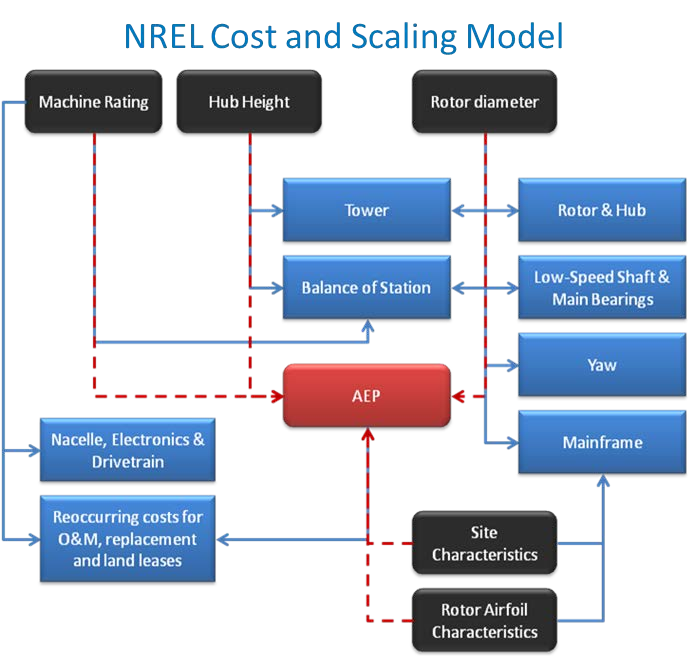
\includegraphics[width=5.5in]{NRELCSM.pdf}
\caption{NREL Cost and Scaling Model Key Input-Output Relationships.}\label{theory:nrelcsm}\end{figure}

The resulting NREL Cost and Scaling Model allows for a variety of interesting analyses including scaling of conventional technology from under a MW to 5 MW+, assessing impact of trends in input factors for materials and labor on wind plant cost of energy, etc.  However, it does not preserve the underlying engineering relationships of the original Sunderland model and thus loses some fidelity of assessing how design changes may impact system costs.

The goal of the development of the following set of models for the hub and nacelle are to return to a semi-empirical physical representation of the turbine that allows one to assess the impact of design changes on dimensions, mass and mass properties while updating the Sunderland model in key areas of limitation related to outdated design criteria.  The resulting models contain two key areas:
\begin{enumerate}
\item {} 
A physical model for sizing each of the major hub and drivetrain components based on design loads as they are transferred through the wind turbine system (tied closely to the Sunderland Model {\hyperref[theory:3]{{[}3{]}}} with some updates for WindPACT work described in {\hyperref[theory:2]{{[}2{]}}} and {\hyperref[theory:4]{{[}4{]}}} and updates for the gearbox and generator in particular based on {\hyperref[theory:5]{{[}5{]}}}).  Using reference {\hyperref[theory:4]{{[}4{]}}}, mass and baseline costs were collected from Table 6-2, p. 39 while final design costs were collected from Table B-2, p. B-2.

\item {} 
A model of the Mass Moments of Inertia for each of the components based on an assumption of homogenous distribution of homogeneous material throughout a simplified geometric structure.  These are necessary for as inputs into a model of overall mass properties for a rotor-nacelle-assembly (RNA) whose properties are fed to an engineering analysis model for the tower.

\end{enumerate}

These models also require an estimate of critical dimensions of each major component.  The dimension estimates as well as some more advanced equations for Mass Moments of Inertia are based on the WindPACT design studies as described in {\hyperref[theory:4]{{[}4{]}}}.  The data on critical dimensions are used in other models such as the balance of station model.

The center of mass for each component is also estimated based on the design studies as described in {\hyperref[theory:4]{{[}4{]}}} and can be used to calculate the aggregate mass properties of the rotor-nacelle-assembly in other models.


\section{Hub System Masses}
\label{theory:hub-system-masses}
The model begins with the Sunderland Model {\hyperref[theory:3]{{[}3{]}}} for the major hub components including the hub itself and the pitch system.  The spinner / nose cone component mass is determined by the NREL Cost and Scaling Model {\hyperref[theory:1]{{[}1{]}}}.  The hub design of the Sunderland model assume a hub with three-fused cylinders rather than a spherical shape as is more common of modern designs.  However, the coefficient multiplier for the hub model was modified from 31.4 to 50 in order to adapt it to data from updated turbine designs of 1 MW+ in size.

The resulting masses from the model can be compared to the estimates from the WindPACT detailed design studies {\hyperref[theory:2]{{[}2{]}}} and the NREL Cost and Scaling Model output.  The below graphs show the mass comparisons for different size turbines of 750 kW, 1 MW, 3 MW and 5 MW for the full hub system as well as each sub-assembly.
\begin{figure}[htbp]
\centering
\capstart

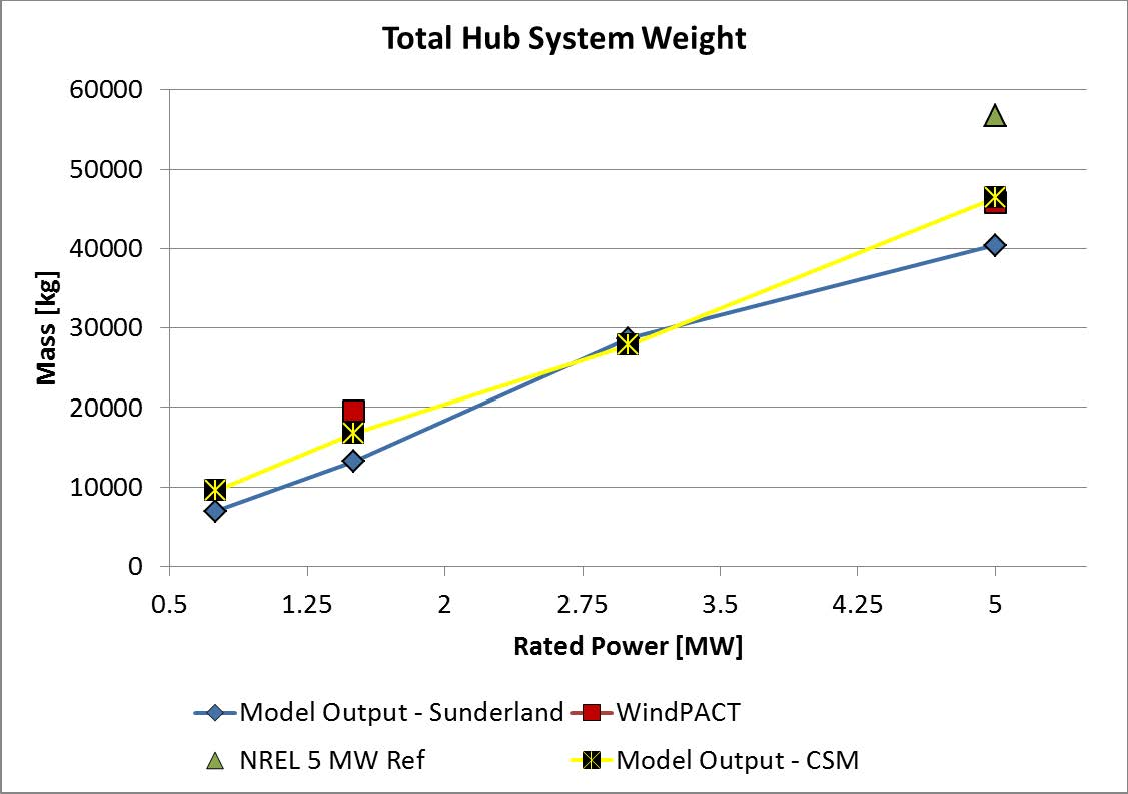
\includegraphics[width=6.5in]{hubsysmass.pdf}
\caption{Hub System overall mass comparison between the NREL Cost and Scaling Model, WindPACT detailed design studies, the NREL 5 MW reference turbine and the NREL Hub System Cost and Sizing Tool.}\label{theory:hubsysmass}\end{figure}
\begin{figure}[htbp]
\centering
\capstart

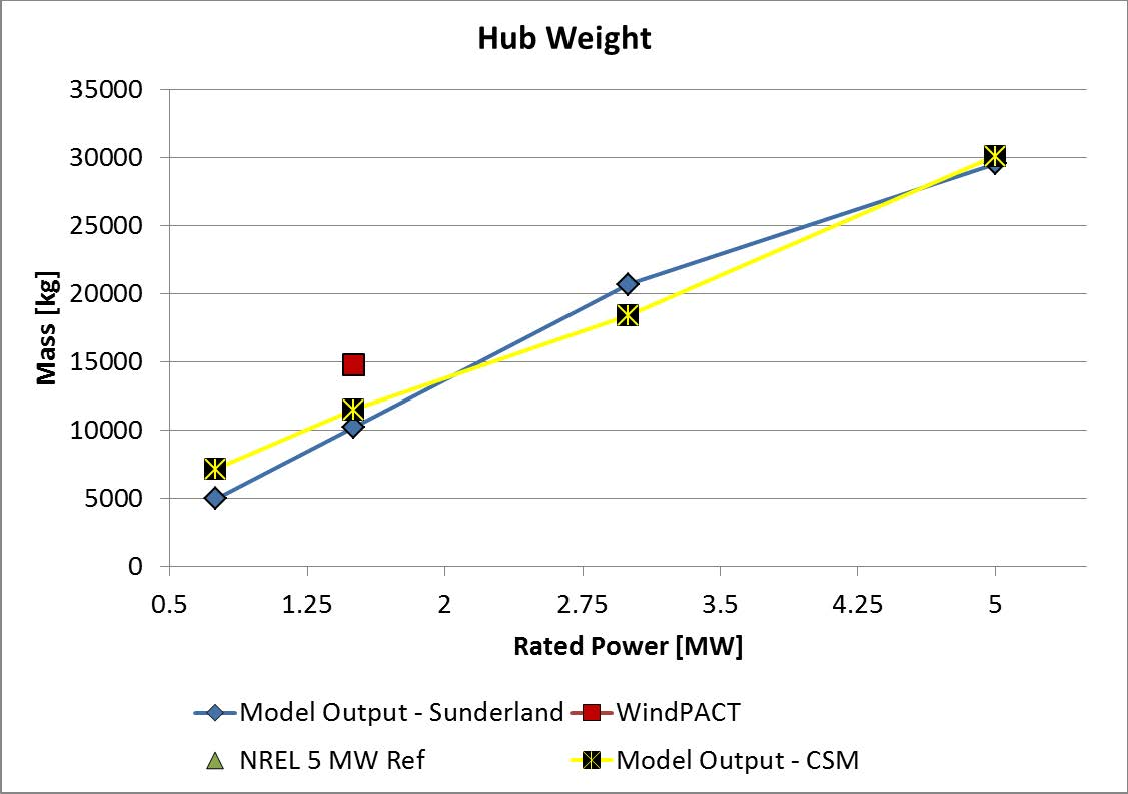
\includegraphics[width=6.5in]{hubmass.pdf}
\caption{Hub component mass comparison between the NREL Cost and Scaling Model, WindPACT detailed design studies, the NREL 5 MW reference turbine and the NREL Hub System Cost and Sizing Tool.}\label{theory:hubmass}\end{figure}
\begin{figure}[htbp]
\centering
\capstart

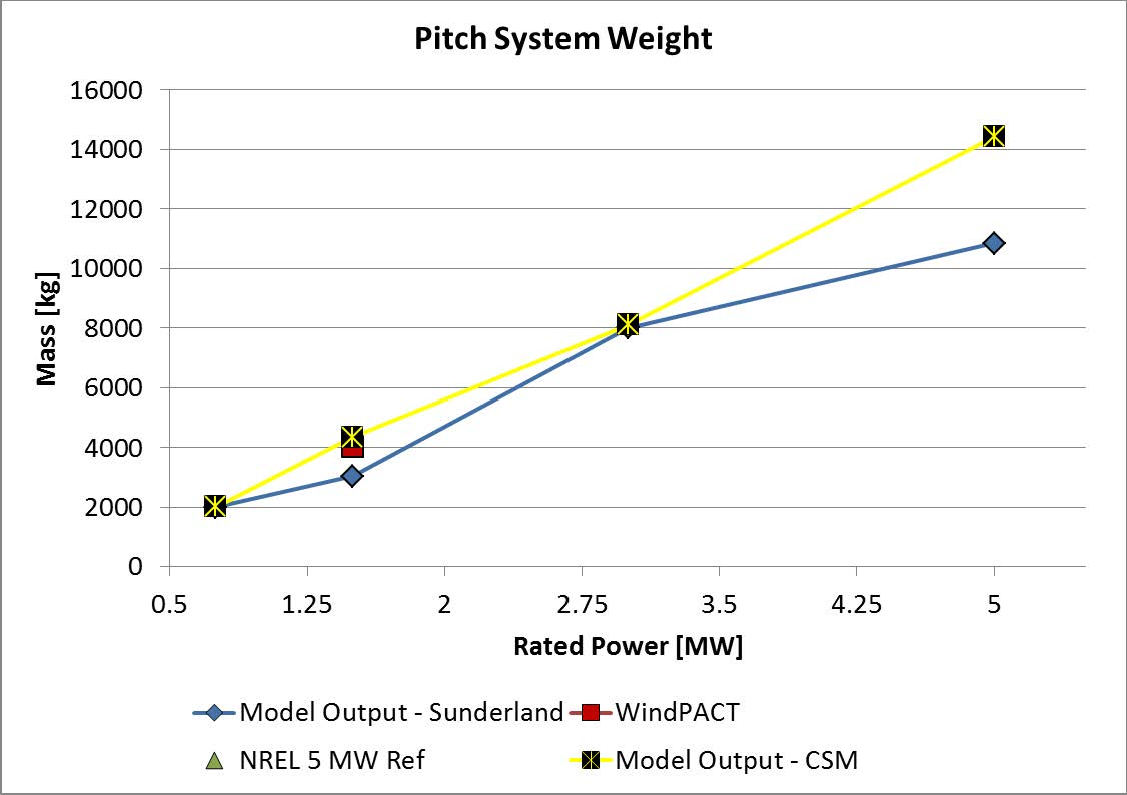
\includegraphics[width=6.5in]{pitchsysmass.pdf}
\caption{Pitch System overall mass comparison between the NREL Cost and Scaling Model, WindPACT detailed design studies, the NREL 5 MW reference turbine and the NREL Hub System Cost and Sizing Tool.}\label{theory:pitchsysmass}\end{figure}
\begin{figure}[htbp]
\centering
\capstart

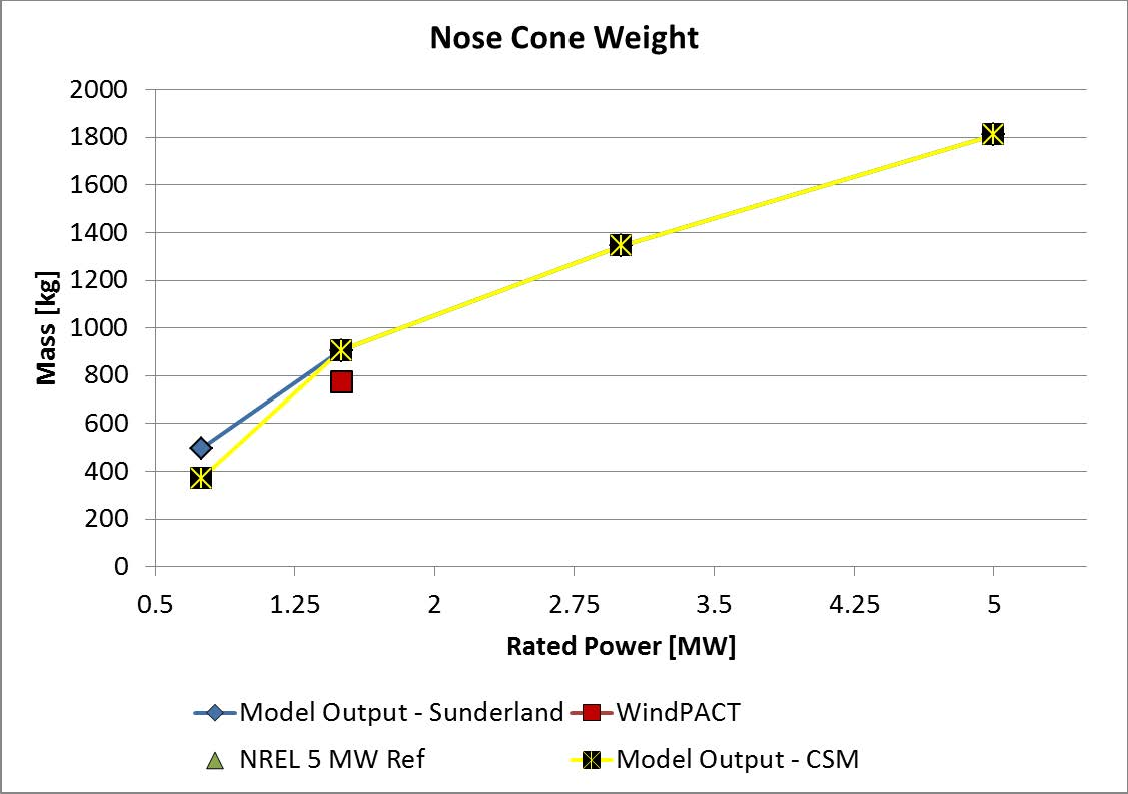
\includegraphics[width=6.5in]{spinnermass.pdf}
\caption{Spinner component mass comparison between the NREL Cost and Scaling Model, WindPACT detailed design studies, the NREL 5 MW reference turbine and the NREL Hub System Cost and Sizing Tool.}\label{theory:spinnermass}\end{figure}

Limitations on data hamper validation efforts but there are also known issues with the models: notably the use of the Sunderland Model as a foundation which was developed based on technology from previous generations.  Still, there is decent agreement between the model output and both the WindPACT study data as well as the NREL Cost and Scaling Model output given the same input spectifications.  Future work will look at updates to the entire set of hub system models so that they are compatible with current technology.


\section{Hub System Mass Moments of Inertia}
\label{theory:hub-system-mass-moments-of-inertia}
For the mass moments of inertia, it is assumed that the hub system is a hollow sphere with its diameter either provided as input or determined as a fraction of the overall rotor diameter.  The thickness is assumed as a fraction of the overall rotor diameter.  The hub and nose cone mass are lumped together in a single quantity while the contribution from the pitch system is modeled as an additional mass about the hub with the hub radius as determined above.  The resulting equation is:
\begin{gather}
\begin{split}I_{xx}=I_{yy}=I_{zz}=2*(hubmass + spinnermass)/5 * (r_{outer}^5 - r_{inner}^5)/(r_{outer}^3 - r_{inner}^3) + pitchmass * r_{outer}^2\end{split}\notag\\\begin{split}\end{split}\notag
\end{gather}
where $I_{xx}$, $I_{yy}$, and $I_{zz}$ are the mass moments of inertia around the respective axis using the wind turbine yaw-aligned coordinate system, $hubmass$, $spinnermass$, and $pitchmass$ are the masses of the hub, spinner and pitch system respectively, and $r_{outer}$ and $r_{inner}$ are the inner and outer radii of the hub respectively.

The center of mass for the hub system is determined relatively to the tower top center as a function of rotor diameter.
\begin{gather}
\begin{split}cm_{x} = -(0.05 * diam)\end{split}\notag\\\begin{split}\end{split}\notag
\end{gather}\begin{gather}
\begin{split}cm_{y} = 0.0\end{split}\notag\\\begin{split}\end{split}\notag
\end{gather}\begin{gather}
\begin{split}cm_{z} = 0.025 * diam\end{split}\notag\\\begin{split}\end{split}\notag
\end{gather}
Where $cm_{x}$,:math:\emph{cm\_\{y\}} and $cm_{z}$ are the positions of center of mass and $diam$ is the rotor diameter of the turbine.


\section{Nacelle Assembly System Masses}
\label{theory:nacelle-assembly-system-masses}
The model begins with the Sunderland Model {\hyperref[theory:3]{{[}3{]}}} for the major nacelle components including the low speed shaft, main bearings, gearbox, high speed shaft, bedplate and yaw system.  The generator component mass is determined by the NREL Cost and Scaling Model {\hyperref[theory:1]{{[}1{]}}} including updates for the drivetrain as described in {\hyperref[theory:5]{{[}5{]}}}.  Some modifications to the models were made where necessary in order to adapt it to data from updated turbine designs of 1 MW+ in size:
\begin{itemize}
\item {} 
The low-speed shaft model includes a mass weight factor of 1.25 which was developed as part of updates as described in {\hyperref[theory:5]{{[}5{]}}}.

\item {} 
The main bearings model includes a mass weight factor of 0.25 to bring the model into closer alignment with {\hyperref[theory:1]{{[}1{]}}}

\item {} 
The gearbox model includes a stage weight factor for each parallel and epicyclic stage.  The stage weight factor for the epicyclic stages has been reduced by a factor of 12.0 to align the model closer to modern gearbox sizes.

\item {} 
The mechanical brake mass is created via a multiplier of 0.5 to the high speed shaft mass to make it consistent with {\hyperref[theory:1]{{[}1{]}}} and {\hyperref[theory:4]{{[}4{]}}}.

\end{itemize}

The models otherwise follow the references and also include the following components (after reference {\hyperref[theory:1]{{[}1{]}}}): variable speed electronics, electrical connections and controls, HVAC system, mainframe platforms, base hardware and crane, and nacelle cover.

The resulting masses from the model can be compared to the estimates from the WindPACT detailed design studies {\hyperref[theory:2]{{[}2{]}}} and the NREL Cost and Scaling Model output.  The below graphs show the mass comparisons for different size turbines of 750 kW, 1 MW, 3 MW and 5 MW for the full hub system as well as each of the modified sub-assemblies: the low-speed shaft, main bearings, gearbox, high-speed shaft and brake, bedplate and yaw system.
\begin{figure}[htbp]
\centering
\capstart

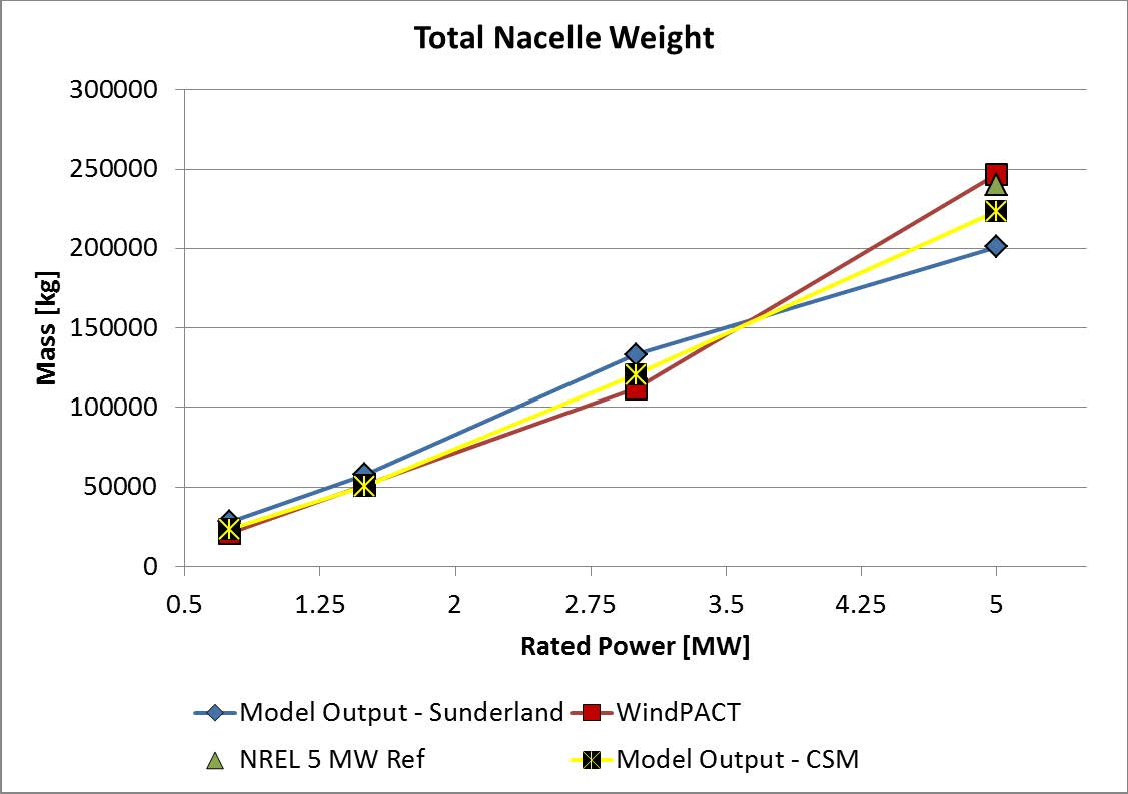
\includegraphics[width=6.5in]{nacellemass.pdf}
\caption{Nacelle overall system mass comparison between the NREL Cost and Scaling Model, WindPACT detailed design studies, the NREL 5 MW reference turbine and the NREL Hub System Cost and Sizing Tool.}\label{theory:nacellemass}\end{figure}
\begin{figure}[htbp]
\centering
\capstart

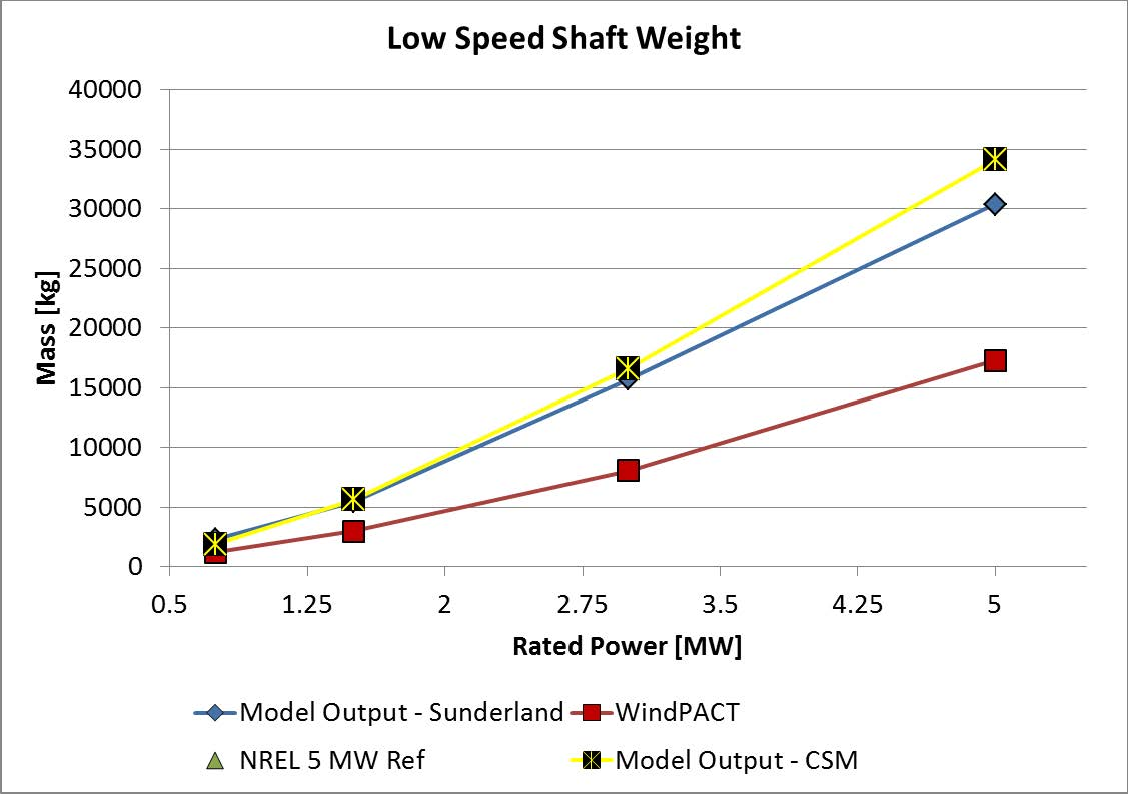
\includegraphics[width=6.5in]{lssmass.pdf}
\caption{LSS component mass comparison between the NREL Cost and Scaling Model, WindPACT detailed design studies, the NREL 5 MW reference turbine and the NREL Hub System Cost and Sizing Tool.}\label{theory:lssmass}\end{figure}
\begin{figure}[htbp]
\centering
\capstart

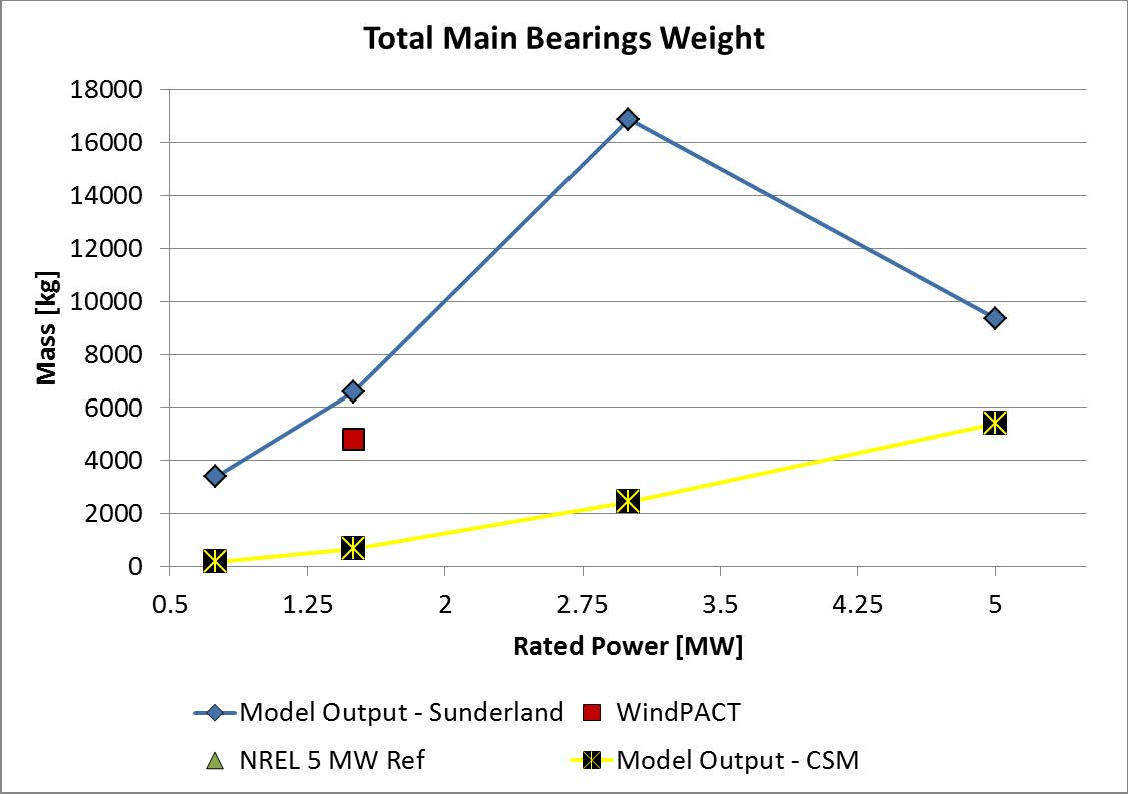
\includegraphics[width=6.5in]{bearingsmass.pdf}
\caption{Main bearing system mass comparison between the NREL Cost and Scaling Model, WindPACT detailed design studies, the NREL 5 MW reference turbine and the NREL Hub System Cost and Sizing Tool.}\label{theory:bearingsmass}\end{figure}
\begin{figure}[htbp]
\centering
\capstart

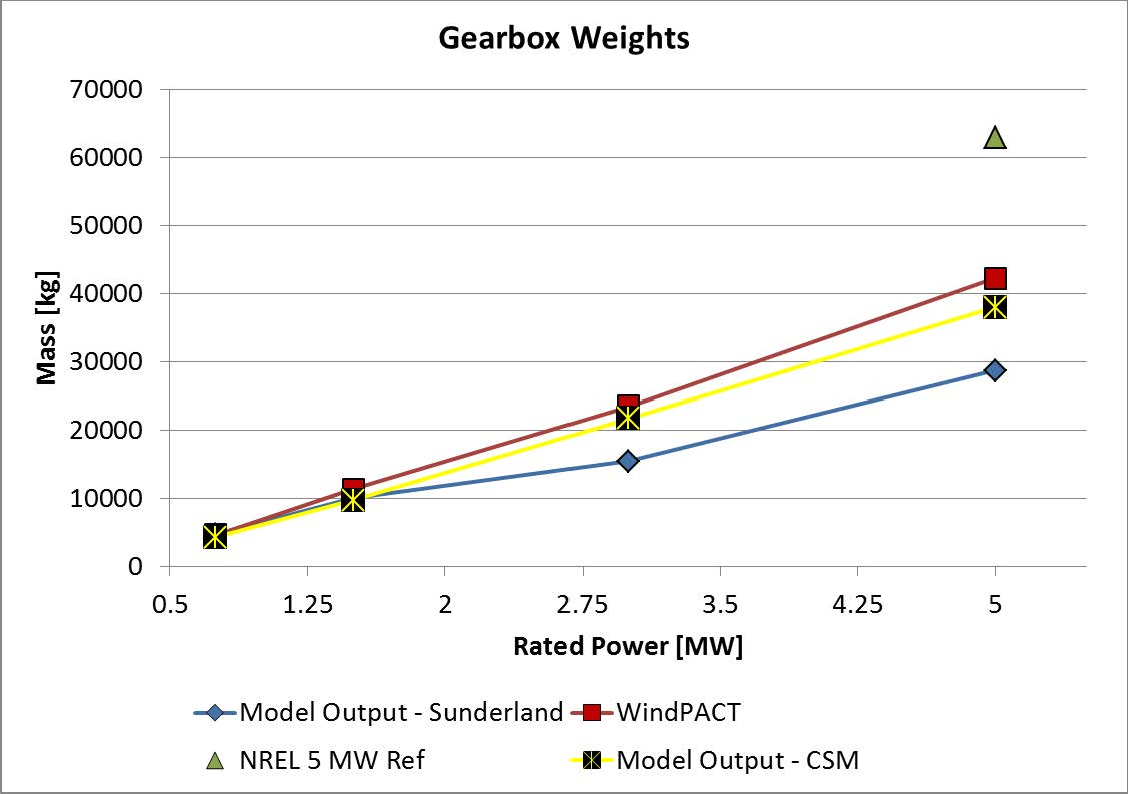
\includegraphics[width=6.5in]{gearboxmass.pdf}
\caption{Gearbox mass comparison between the NREL Cost and Scaling Model, WindPACT detailed design studies, the NREL 5 MW reference turbine and the NREL Hub System Cost and Sizing Tool.}\label{theory:gearboxmass}\end{figure}
\begin{figure}[htbp]
\centering
\capstart

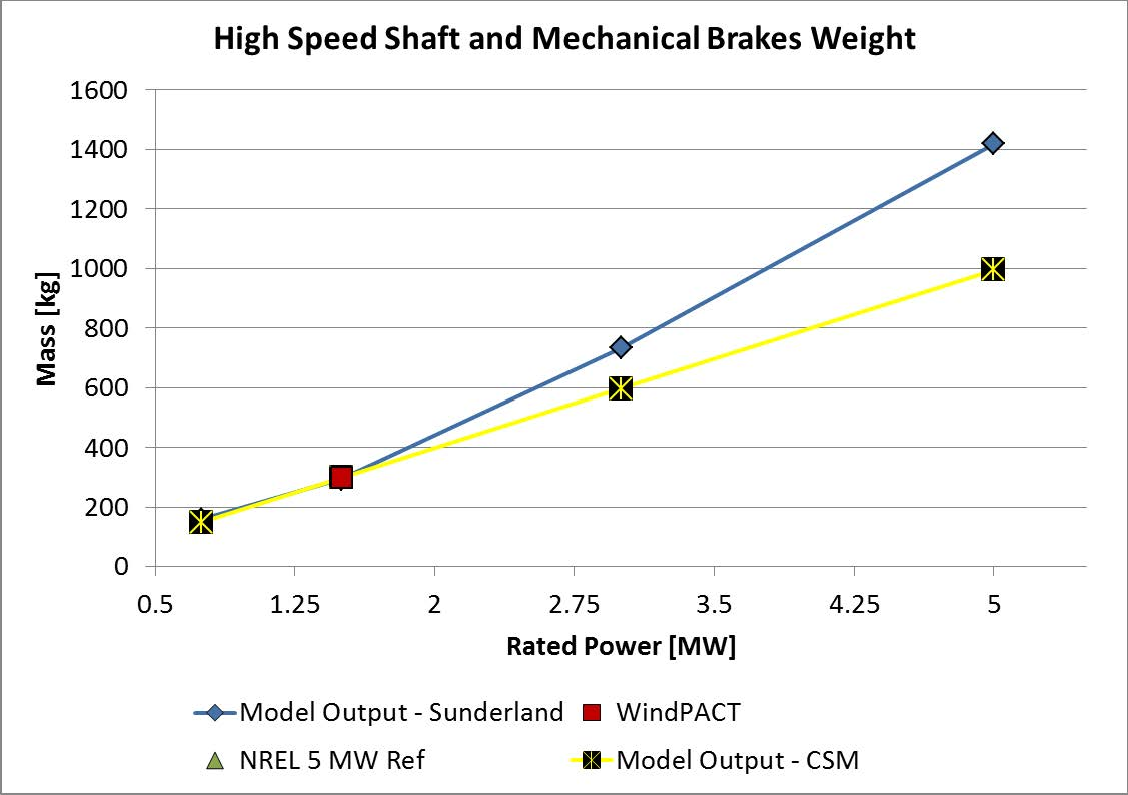
\includegraphics[width=6.5in]{hssmass.pdf}
\caption{HSS and brake component overall mass comparison between the NREL Cost and Scaling Model, WindPACT detailed design studies, the NREL 5 MW reference turbine and the NREL Hub System Cost and Sizing Tool.}\label{theory:hssmass}\end{figure}
\begin{figure}[htbp]
\centering
\capstart

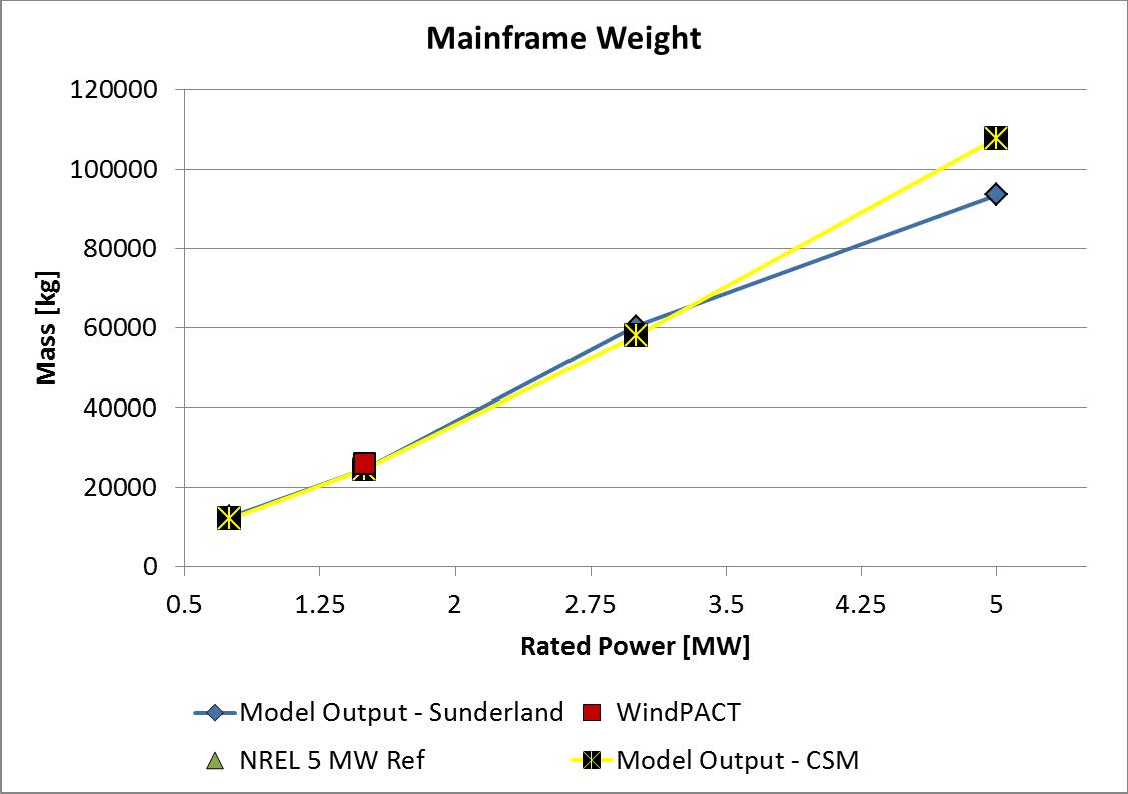
\includegraphics[width=6.5in]{bedplatemass.pdf}
\caption{Bedplate mass comparison between the NREL Cost and Scaling Model, WindPACT detailed design studies, the NREL 5 MW reference turbine and the NREL Hub System Cost and Sizing Tool.}\label{theory:bedplatemass}\end{figure}
\begin{figure}[htbp]
\centering
\capstart

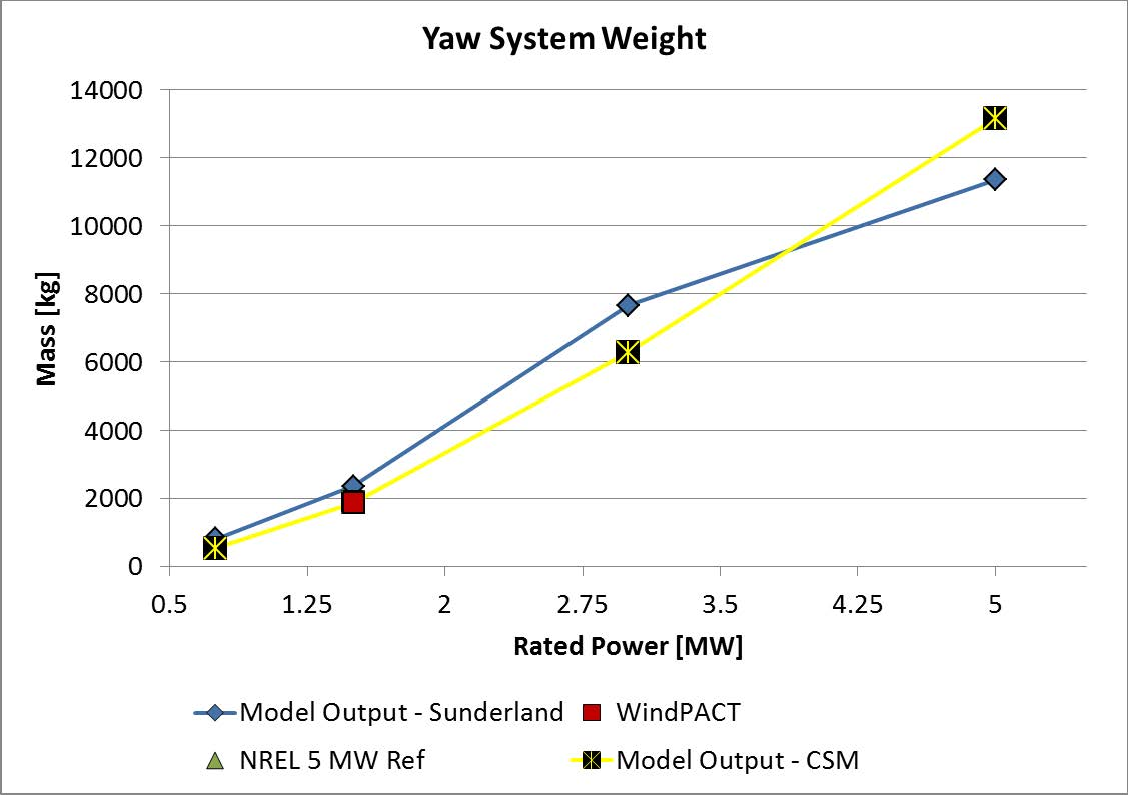
\includegraphics[width=6.5in]{yawmass.pdf}
\caption{Yaw system mass comparison between the NREL Cost and Scaling Model, WindPACT detailed design studies, the NREL 5 MW reference turbine and the NREL Hub System Cost and Sizing Tool.}\label{theory:yawmass}\end{figure}

Limitations on data hamper validation efforts but there are also known issues with the models: notably the use of the Sunderland Model as a foundation which was developed based on technology from previous generations.  Still, there is decent agreement between the model output and both the WindPACT study data as well as the NREL Cost and Scaling Model output given the same input spectifications.  Future work will look at updates to the entire set of nacelle assembly models so that they are compatible with current technology.


\section{Nacelle Assembly Mass Moments of Inertia}
\label{theory:nacelle-assembly-mass-moments-of-inertia}
For the mass moments of inertia, it is assumed that basic geometric shapes with homogeneous distribution of homogenous materials are assumed.  Each major component has its own set of calculations.  The assumptions regarding the shape of components is based on the design studies as described in {\hyperref[theory:2]{{[}2{]}}}.

Low Speed Shaft:

The low speed shaft is assumed to be a hollow-cylinder along the yaw-aligned x-axis.  The resulting equations are:
\begin{gather}
\begin{split}I_{xx}=lssmass * (r_{outer}^2 + r_{inner}^2) / 8\end{split}\notag\\\begin{split}\end{split}\notag
\end{gather}\begin{gather}
\begin{split}I_{yy}=I_{zz}=lssmass * (r_{outer}^2 + r_{inner}^2 + (4/3) * lsslength^2)) / 16\end{split}\notag\\\begin{split}\end{split}\notag
\end{gather}
where $I_{xx}$, $I_{yy}$, and $I_{zz}$ are the mass moments of inertia around the respective axis using the wind turbine yaw-aligned coordinate system, $lssmass$ is the mass of the low speed shaft, $lsslength$ is the length of the shaft, and $r_{outer}$ and $r_{inner}$ are the inner and outer radii of the hub respectively.

The center of mass for the low speed shaft is determined relatively to the tower top center as a function of rotor diameter.
\begin{gather}
\begin{split}cm_{x} = -(0.035 ? 0.1) * diam\end{split}\notag\\\begin{split}\end{split}\notag
\end{gather}\begin{gather}
\begin{split}cm_{y} = 0.0\end{split}\notag\\\begin{split}\end{split}\notag
\end{gather}\begin{gather}
\begin{split}cm_{z} = 0.025 * diam\end{split}\notag\\\begin{split}\end{split}\notag
\end{gather}
Where $cm_{x}$,:math:\emph{cm\_\{y\}} and $cm_{z}$ are the positions of center of mass and $diam$ is the rotor diameter of the turbine.

Main bearings:

The main bearings and their housings are assumed to be hoops along the yaw-aligned x-axis with a bearing hoop radius equal to the outer diameter of the low speed shaft and a housing hoop radius equal to a multiplier of the bearing radius of 1.5.  The resulting equations are:
\begin{gather}
\begin{split}I_{xx}=(bearingmass * (r_{bearing}^2) / 4) + (housingmass * (r_{housing}^2) / 4)\end{split}\notag\\\begin{split}\end{split}\notag
\end{gather}\begin{gather}
\begin{split}I_{yy}=I_{zz}=I_{xx}/2\end{split}\notag\\\begin{split}\end{split}\notag
\end{gather}
Where $bearingmass$ and $housingmass$ are the mass of an individual main bearing and its housing respectively, $lsslength$ is the length of the shaft, and $r_{bearing}$ and $r_{housing}$ are the radii of the bearing and its housing respectively.

The center of mass for the main bearing is determined relatively to the tower top center as a function of rotor diameter.
\begin{gather}
\begin{split}cm_{x} = -(0.035 * diam)\end{split}\notag\\\begin{split}\end{split}\notag
\end{gather}\begin{gather}
\begin{split}cm_{y} = 0.0\end{split}\notag\\\begin{split}\end{split}\notag
\end{gather}\begin{gather}
\begin{split}cm_{z} = 0.025 * diam\end{split}\notag\\\begin{split}\end{split}\notag
\end{gather}
The center of mass for the second bearing is determined relatively to the tower top center as a function of rotor diameter.
\begin{gather}
\begin{split}cm_{x} = -(0.01 * diam)\end{split}\notag\\\begin{split}\end{split}\notag
\end{gather}\begin{gather}
\begin{split}cm_{y} = 0.0\end{split}\notag\\\begin{split}\end{split}\notag
\end{gather}\begin{gather}
\begin{split}cm_{z} = 0.025 * diam\end{split}\notag\\\begin{split}\end{split}\notag
\end{gather}
Gearbox:

The gearbox is assumed to be a solid cylinder while the housing is a hollow cylinder along the yaw-aligned x-axis.  The radius of the gearbox is proportional to the housing height.  The resulting equations is:
\begin{gather}
\begin{split}I_{xx}=(gearboxmass * diameter^2 / 8)+ (gearboxmass/2 * height^2 / 8)\end{split}\notag\\\begin{split}\end{split}\notag
\end{gather}\begin{gather}
\begin{split}I_{yy}=I_{zz}= gearboxmass * (0.5 * diameter^2 + (2/3) * length^2 + (1/4) * height^2) / 8\end{split}\notag\\\begin{split}\end{split}\notag
\end{gather}
where $gearboxmass$ is the mass of the gearbox, $length$ is the length of the gearbox, and $diameter$ and $height$ are the radii of the gearbox diameter and height respectively.

The center of mass for the gearbox is determined relatively to the tower top center as a function of rotor diameter.
\begin{gather}
\begin{split}cm_{x} = 0.0\end{split}\notag\\\begin{split}\end{split}\notag
\end{gather}\begin{gather}
\begin{split}cm_{y} = 0.0\end{split}\notag\\\begin{split}\end{split}\notag
\end{gather}\begin{gather}
\begin{split}cm_{z} = 0.025 * diam\end{split}\notag\\\begin{split}\end{split}\notag
\end{gather}
High Speed Shaft and Brake:

The high speed shaft is neglected and the brake disk is used for calculations as roughly a cylinder along the yaw-aligned x-axis.  The calculation, however, deviate for math:\emph{I\_\{xx\}}.  The resulting equations are:
\begin{gather}
\begin{split}I_{xx}=(1/4) * length * pi * diameter^2 * gearratio * diameter^2) / 8\end{split}\notag\\\begin{split}\end{split}\notag
\end{gather}\begin{gather}
\begin{split}I_{yy}=I_{zz}= hssmass * ((3/4) * diameter^2 + length^2) / 12\end{split}\notag\\\begin{split}\end{split}\notag
\end{gather}
Where $hssmass$ is the mass of the high speed shaft and brake, $lsslength$ is the length of the brake, and $diameter$ is the diameter of the low speed shaft, and $gearratio$ is the high-speed to low speed shaft ratio.

The center of mass for the low speed shaft is determined relatively to the tower top center as a function of rotor diameter.
\begin{gather}
\begin{split}cm_{x} = 0.5 * (0.0125 * diam)\end{split}\notag\\\begin{split}\end{split}\notag
\end{gather}\begin{gather}
\begin{split}cm_{y} = 0.0\end{split}\notag\\\begin{split}\end{split}\notag
\end{gather}\begin{gather}
\begin{split}cm_{z} = 0.025 * diam\end{split}\notag\\\begin{split}\end{split}\notag
\end{gather}
Generator:

The generator housing is treated as a hollow cylinder along the yaw-aligned x-axis.  However, the rotating inertia is also approximated and this has a significant impact on the the calculations for math:\emph{I\_\{xx\}}.  The resulting equations are:
\begin{gather}
\begin{split}I_{xx}=((4.86 * 10^-5) * diameter^5.333) + ((2/3) * generatormass * (depth^2 + width^2))/8\end{split}\notag\\\begin{split}\end{split}\notag
\end{gather}\begin{gather}
\begin{split}I_{yy}=I_{zz}= (I_{xx}/2)/(gearratio^2) + ((1/3) * generatormass * length^2 / 12) + ((2/3) * generatormass * (depth^ 2 + width^2 + (4/3)*length^2) / 16)\end{split}\notag\\\begin{split}\end{split}\notag
\end{gather}
Where $generatormass$ is the mass of the generator and housing, $lsslength$ is the length of the housing, $width$ is the width and $height$ is the height, $gearratio$ is the high-speed to low speed shaft ratio, and $diam$ is the overall turbine rotor diameter as before.

The center of mass for the low speed shaft is determined relatively to the tower top center as a function of rotor diameter.
\begin{gather}
\begin{split}cm_{x} = 0.0125 * diam\end{split}\notag\\\begin{split}\end{split}\notag
\end{gather}\begin{gather}
\begin{split}cm_{y} = 0.0\end{split}\notag\\\begin{split}\end{split}\notag
\end{gather}\begin{gather}
\begin{split}cm_{z} = 0.025 * diam\end{split}\notag\\\begin{split}\end{split}\notag
\end{gather}
Bedplate:

Finally, the bedplate is modeled as a hollow cylinder along the yaw-aligned x-axis.  The resulting equations are:
\begin{gather}
\begin{split}I_{xx}=bedplatemass * (width^2 + depth^2) / 8\end{split}\notag\\\begin{split}\end{split}\notag
\end{gather}\begin{gather}
\begin{split}I_{yy}=I_{zz}=bedplatemass * (width^2 + depth^2 + (4/3)*length^2) / 16\end{split}\notag\\\begin{split}\end{split}\notag
\end{gather}
Where $bedplatemass$ is the mass of the bedplate, $length$ is the length of the housing, $width$ is the width, and $depth$ is the depth.

The center of mass for the low speed shaft is determined relatively to the tower top center as a function of rotor diameter.
\begin{gather}
\begin{split}cm_{x} = 0.0\end{split}\notag\\\begin{split}\end{split}\notag
\end{gather}\begin{gather}
\begin{split}cm_{y} = 0.0\end{split}\notag\\\begin{split}\end{split}\notag
\end{gather}\begin{gather}
\begin{split}cm_{z} = 0.0122 * diam\end{split}\notag\\\begin{split}\end{split}\notag
\end{gather}
Other components:

The other masses in the system are small compared to the major drivetrain components and are ignored for the purposes of calculating overall center of mass and mass moments of inertia for the nacelle assembly.



\begin{thebibliography}{1}
\bibitem[1]{1}{\phantomsection\label{theory:1} \DUspan{}{\DUspan{}{\DUspan{}{\DUspan{}{\DUspan{}{\DUspan{}{\DUspan{}{\DUspan{}{L.}\DUspan{}{ }}\DUspan{}{Fingersh}}\DUspan{}{, }\DUspan{}{\DUspan{}{\DUspan{}{M.}\DUspan{}{ }}\DUspan{}{Hand}}}\DUspan{}{, and }\DUspan{}{\DUspan{}{\DUspan{}{A.}\DUspan{}{ }}\DUspan{}{Laxson}}}\DUspan{}{.}}\DUspan{}{ }\DUspan{}{\DUspan{}{Wind turbine design cost and scaling model}\DUspan{}{.}}}\DUspan{}{ }\DUspan{}{\DUspan{}{\DUspan{}{NREL/TP-500-40566}\DUspan{}{, }\DUspan{}{National Renewable Energy Laboratory}\DUspan{}{, }\DUspan{}{Golden, CO}}\DUspan{}{, }\DUspan{}{\DUspan{}{December}\DUspan{}{ }\DUspan{}{2005}}\DUspan{}{.}}}}
\bibitem[2]{2}{\phantomsection\label{theory:2} \DUspan{}{\DUspan{}{\DUspan{}{WindPACT}\DUspan{}{.}}\DUspan{}{ }\DUspan{}{\DUspan{}{Wind partnerships for advanced component technology (windpact)}\DUspan{}{.}}}}
\bibitem[3]{3}{\phantomsection\label{theory:3} \DUspan{}{\DUspan{}{\DUspan{}{\DUspan{}{\DUspan{}{\DUspan{}{\DUspan{}{R.}\DUspan{}{ }}\DUspan{}{Harrison}}\DUspan{}{ and }\DUspan{}{\DUspan{}{\DUspan{}{G.}\DUspan{}{ }}\DUspan{}{Jenkins}}}\DUspan{}{.}}\DUspan{}{ }\DUspan{}{\DUspan{}{Cost modeling of horizontal axis wind turbines}\DUspan{}{.}}}\DUspan{}{ }\DUspan{}{\DUspan{}{\DUspan{}{ETSU/W-34-00170-REP}\DUspan{}{, }\DUspan{}{University of Sunderland, School of Environment}\DUspan{}{, }\DUspan{}{Sunderland, UK}}\DUspan{}{, }\DUspan{}{\DUspan{}{December}\DUspan{}{ }\DUspan{}{1993}}\DUspan{}{.}}}}
\bibitem[4]{4}{\phantomsection\label{theory:4} \DUspan{}{\DUspan{}{\DUspan{}{\DUspan{}{\DUspan{}{\DUspan{}{\DUspan{}{D.J.}\DUspan{}{ }}\DUspan{}{Malcolm}}\DUspan{}{ and }\DUspan{}{\DUspan{}{\DUspan{}{A.C.}\DUspan{}{ }}\DUspan{}{Hansen}}}\DUspan{}{.}}\DUspan{}{ }\DUspan{}{\DUspan{}{Windpact turbine rotor design study}\DUspan{}{.}}}\DUspan{}{ }\DUspan{}{\DUspan{}{\DUspan{}{NREL/SR-500-32495}\DUspan{}{, }\DUspan{}{National Renewable Energy Laboratory}\DUspan{}{, }\DUspan{}{Golden, CO}}\DUspan{}{, }\DUspan{}{\DUspan{}{April}\DUspan{}{ }\DUspan{}{2006}}\DUspan{}{.}}}}
\bibitem[5]{5}{\phantomsection\label{theory:5} \DUspan{}{\DUspan{}{\DUspan{}{\DUspan{}{\DUspan{}{\DUspan{}{\DUspan{}{\DUspan{}{B.}\DUspan{}{ }}\DUspan{}{Maples}}\DUspan{}{, }\DUspan{}{\DUspan{}{\DUspan{}{M.}\DUspan{}{ }}\DUspan{}{Hand}}}\DUspan{}{, and }\DUspan{}{\DUspan{}{\DUspan{}{W.}\DUspan{}{ }}\DUspan{}{Musial}}}\DUspan{}{.}}\DUspan{}{ }\DUspan{}{\DUspan{}{Comparative assessment of direct drive high temperature superconducting generators in multi-megawatt class wind turbines}\DUspan{}{.}}}\DUspan{}{ }\DUspan{}{\DUspan{}{\DUspan{}{NREL/TP-5000-49086}\DUspan{}{, }\DUspan{}{National Renewable Energy Laboratory}\DUspan{}{, }\DUspan{}{Golden, CO}}\DUspan{}{, }\DUspan{}{\DUspan{}{October}\DUspan{}{ }\DUspan{}{2010}}\DUspan{}{.}}}}
\end{thebibliography}



\end{document}
